%\begin{comment}

\documentclass[a4paper, 12pt]{article}
\setlength{\parindent}{4ex}
\usepackage{natbib}
\bibliographystyle{apa}
\usepackage{amsmath,amssymb,amsfonts,amsthm, amstext}    
\usepackage{graphicx,subcaption} 
%\usepackage[list=true]{subcaption} 
%\usepackage{subfig}
\usepackage{hyperref}                          
\usepackage[font = bf, labelfont = bf]{caption}
\usepackage{url}
\usepackage{appendix}
\usepackage{pdflscape}
\usepackage{booktabs}
\usepackage{longtable}
\usepackage{xcolor}
\usepackage{tikz}
\usepackage{float}
\usepackage[onehalfspacing]{setspace}
\usepackage{breqn}
\usepackage{tabu}
\usepackage{indentfirst}
\usepackage{fullpage}
\usepackage{comment}
\usepackage{array}   % for \newcolumntype macro
\newcolumntype{C}{>{$}c<{$}} % math-mode version of "l" column type
\usepackage[automark]{scrpage2}
\usepackage{multirow}
\usepackage{footnote}
\usepackage{enumitem}
\usepackage{nicefrac}
\usepackage{dsfont}
\usepackage{multirow}
\makesavenoteenv{tabular}
\pagestyle{scrheadings}
\automark{section}
\clearscrheadings
\ohead{\headmark}

\setlength{\headheight}{1.1\baselineskip}
\voffset=-2cm 
\hoffset=-3cm
\textheight24cm
\textwidth15.5cm
\topmargin1cm
\oddsidemargin3cm
\evensidemargin3cm
\makeatletter
%\setlength{\@fptop}{0pt}
\makeatother
%%%%%%%%%%%%%%%%%%%%%%%%%%%%%%%%%%%%%%%%%%%%
\begin{document}
\thispagestyle{empty}
\begin{center} 

%{\Large{\bf Sex and education model: \\Characterizing the HIV epidemic} 
%\vspace{2cm}\\
%\Large {by} \\ 
%\vspace{0.25cm}
%{\bf Christian Aleman} \\
%\vspace{1cm}
%{} Barcelona, \today} \\

\Large{
\textbf{Sex and education model}\\
\vspace{0.5cm}
\Large {by}\\  
\vspace{0.25cm}
\textbf{Raul Santaeulalia Llopis}\\
\vspace{0.25cm}
%\large{Advisor\\
%\vspace{0.25cm}
\textbf{Daniela Iorio}\\
\vspace{0.25cm}
\textbf{Christian Aleman}\\
}
\vspace{0.7cm}
%\Large{
%\Large{Master project submitted in partial satisfaction of the requirements for the degree Master in Models and Methods of Quantitative Economics}\\
\vspace{0.7cm}
%Barcelona,\,\,\today} \\
Barcelona,\,\,\today \\
\vspace{0.3cm}
%\textbf{IDEA-QEM}		
    
   %Better example of title see Christoph Schult technical report

  
\end{center}



   %Better example of title see Christoph Schult technical report

  

\vspace{2cm}
\begin{center}
\Large{\bf{Abstract}}\\
\end{center}
\indent In this paper I examine the role of education on the evolution of the exposure to HIV risk across the HIV epidemic. Cross country empirical results show that the education gradient in HIV is U-shaped. This means that at some point during the HIV epidemic, agents with higher education have a higher risk of becoming HIV positive. I propose a heterogeneous agent general equilibrium model to account for this stylized fact. Additionally, the paper proposes an algorithm to fully characterize the evolution of the HIV epidemic across stages.  The model is calibrated to match the prevalences of the Malawian HIV epidemic. Finally, using the data generated by the model I calculate the education gradient for Malawi, the results show that the shape of the education gradient is in line with the empirical evidence. The model paves the road further policy implications, for example targeted prevention depending on the stage of the HIV epidemic. 
%\footnote{The attached MATLAB code 'Laffer_curve_Bolivia.m' contains the solution of the model,the main results and graphs}.


\pagenumbering{roman}

\begin{comment}
\newpage
\singlespacing
\tableofcontents
\onehalfspacing
\clearpage
\pagenumbering{roman}   % define page number in roman style
\setcounter{page}{1}    % start page numbering
\newpage
\addcontentsline{toc}{section}{List of Tables}
\listoftables
\addcontentsline{toc}{section}{List of Figures}
\listoffigures
\end{comment}

\newpage
\pagestyle{plain}
\setcounter{page}{1}    % start page numbering anew
\pagenumbering{arabic}  % page numbers in arabic style

\section{Introduction}\label{sec1}

Targeted prevention suggests that irrespective of the stage of the epidemic an efficient way to reduce HIV diffusion is to target the groups at high risk. As described by the \cite{report2} report, certain groups have a higher chance to get and spread HIV. These groups include mostly individuals engaging in high-risk sexual behavior such as sex workers and their clients, injecting drug users and recently, men who have sex with men. How about individuals across educational groups?\\

\cite{beegle} argue that there is a lack of consensus on the sign and the size of the relationship between education and HIV exposure, in other words, it is still not clear if people with lower education have a higher risk of infection or if its the other way around. \cite{raul} provides empirical evidence on the relationship between HIV status and education. He finds that risky sex behavior (associated with high HIV exposure), differs across educational groups as the HIV epidemic evolves. In particular, the education gradient in HIV has a U shape across the HIV epidemic. This means that in the early stages of the epidemic, additional years of education are associated with an increase of the probability of being HIV infected. This fact is the main motivation for this paper.   \\

This paper proposes a general equilibrium model that studies extramarital risky sex and its implications for HIV diffusion. The model treats the market of extramarital risky sex as any other competitive market, in which agents pay a competitive price and consume an amount of the desired good. In the model, agents are heterogeneous and differ principally in their education level and their level of asset holdings. Agents can be of two types: sex buyers or sex producers. In the model, the probability of HIV infection depends on the amount of extramarital risky sex an individual consumes. That is, the infection probability is endogenously determined by the model. In principle, agents are infinitely lived, however they have a random  probability of dying. Additionally, population grows at a constant rate.\\ %This eliminated from chris. Dont do it for the thesis.
%\section{The model}\label{sec4}
This section describes the proposed heterogeneous agent general equilibrium model.
\subsection{Model characteristics}
The model features two types agents: sex consumers and sex producers. They are finitely lived, have rational expectations and intend to maximize future discounted utility, $E_{0}\sum_{t}^{\infty}\beta^{t}u$, subject to their respective budget constraints. I assume the function $u:[0,\infty)\to \mathbb{R}$ is strictly increasing, strictly concave and twice continuously differentiable. \\
 Agents interact in three competitive markets in this economy: The goods market, the sex market and the assets market.  
\begin{itemize}
\item From the goods market agents can obtain consumption good $c$ at price $p_{1}$\footnote{From now on I will use the price of the consumption good as numeraire, then $p_{1}=1$}. 
\item Non-marital risky sex $x$ is traded in the sex market for price $p_{2}=p$. Where variable $x$ is continuous.
\item Individuals can either save or borrow in the asset market by trading a non-contingent asset $a$ with endogenous return $r$.
\item Agents education can either be high or low $e=\{1,0\}$.
\item HIV status can be positive or negative $h=\{1,0\}$.
\item Labor is supplied inelastically.
\item Agents receive labor income $y(e)$, where income differs according to their education level $e$. In particular $y(1)>y(0)$.
\item Let $\gamma_{e}$ denote the survival probability of an agent with level of education $e$.
\item Let $\psi^{h}$ be the fertility rate of an individual with HIV status $h$.
\item Let $\lambda(x,h)$ denote the probability of getting infected with HIV. Note that the probability of infection is actually a function of the amount of risky sex($x$) consumed by the agent. This value is determined endogenously.
\item There are two types of agents sex buyers ($g$) and sex producers ($-g$).  
\end{itemize}
Following the discussion in Section\ref{sec1}, the model intends to characterize the different stages of the HIV epidemic according to the level of education of the population. In particular, the increase in the probability of infection for the most educated in the early and final stages.\\
In line with \cite{raul}, four stages of the epidemic have been identified. 
\begin{enumerate}
\item Pre-Epidemic stage
\item Miopic stage of the epidemic
\item Difussion and maturity of the epidemic
\item Introduction of anti-retro viral drugs
\end{enumerate}
The features of each stage will be described in detail in the upcoming sections.\\

The model features additional dynamics, in the sense that it intends to capture the evolution of the HIV epidemic starting from stage one until stage four. For presentation purposes each stage characterizes a stationary equilibrium, but later on they will be linked with the intention to describe the complete evolution of the HIV epidemic.

In the following sections I describe in detail the characteristics of each of the stages of the model.  
\subsection{Pre-epidemic stage}\label{pre}
In this pre-HIV world, there is no probability of infection, namely $\lambda_(x,h)=0$. Agents differ on their type $g$, assets $a$ and education level $e$.\\

\noindent\textbf{Sex Buyers:}\\
For agents of type $g$ the dynamic problem is:
\begin{align}
V(a,e,g;\Phi) &= \mathop{\max_{c\geq 0,x \geq 0,a' \geq 0}}  u(c,x) + \beta \gamma_{e} V(a',e,g;\Phi') \label{eq1}\\
\mbox{s.t}\nonumber\\
c+ px +a'&= y(e) + (1+r(\Phi))a \label{eq2}
\end{align}

 Agents interact in non-marital risky sex activities, these agents buys non-marital risky sex $x$ at price $p$ and saves or borrows $a'$ with return $r$. Note that labor is supplied inelastically and depends on their level of education $e$, then their labor income is $y(e)$, where $y(1)>y(0)$.\\
 This problem is characterized by three individual state variables ($a,e,g$) and one aggregate state variable $\Phi$, which represents the population distribution over the states $a,e,g$. The choice variables are $c,x$ and $a'$.\\
The above problem can be written in sequential form: 
\begin{align*}
\mathop{\max_{c_{t},x_{t},a_{t+1}}}&E_{0}\sum^{\infty}_{t=0}\beta^{t}u(c_{t},x_{t})  \\
\mbox{s.t}\\ 
c_{t}+p_{t}x_{t}+a_{t+1}&=y(e)+(1+r_{t})a_{t}
\end{align*}
 \textbf{FOC's:}\\
 \begin{align*}
 \frac{\partial u(c_{t},x_{t})}{\partial x_{t}}&=-u'_{c}(c_{t},x_{t})p_{t}+u'_{x}(c_{t},x_{t})=0\\
 \frac{\partial u(c_{t},x_{t})}{\partial a_{t+1}}&=-u'_{c}(c_{t},x_{t})+u'_{c}(c_{t+1},x_{t+1})(1+r_{t})\beta=0
 \end{align*}
 Given the price system $\{p_{t}\}_{t=0}^{\infty},\{r_{t}\}_{t=0}^{\infty}$ the solution is characterized by the sequence of allocations $\{c_{t}\}_{t=0}^{\infty}, \{x_{t}\}_{t=0}^{\infty}, \{a_{t}\}_{t=0}^{\infty}$ such that they solve the above maximization problem.\\
 
\noindent \textbf{Sex Producers:}\\
For agents of type $-g$ the dynamic problem is:
\begin{align}
V(a,e,-g;\Phi) &= \mathop{\max_{c\geq 0, 1\geq l\geq 0,a' \geq 0}}  u(c) + \beta \gamma_{e} V(a',e,-g;\Phi') \label{eq3}\\
\mbox{s.t}\nonumber\\
c +a'&= pl^{\alpha}+y(e)(1-l) + (1+r(\Phi))a \label{eq4}
\end{align}
Note that for these agents, extra marital risky sex does not generate any utility, then the utility function only depends on the amount of $c$ consumed. Additionally, these agents produce sex with a decreasing return to scale production function $x=l^{\alpha}$ where $\alpha\in(0,1)$. In other words, these agents produce non-marital risky-sex $x$ using time $l$ and sell it a price $p$. Where $l$ is the fraction of labor dedicated to the production of sex, the rest of the labor ($1-l$) which is not allocated to sex production is sold in the market for labor income $y(e)$. Additionally agents save or borrow assets $a$ at rate $r$.\\

\noindent The above problem can be written in sequential form: 
\begin{align*}
\mathop{\max_{c_{t},l_{t},a_{t+1}}}&E_{0}\sum^{\infty}_{t=0}\beta^{t}u(c_{t})  \\
\mbox{s.t}\\ 
c_{t}+a_{t+1}&=p_{t}l_{t}^{\alpha}+y(e)(1-l_{t})+(1+r_{t})a_{t}
\end{align*}
 \textbf{FOC's:}\\
 \begin{align*}
 \frac{\partial u(c_{t})}{\partial l_{t}}&=-u'_{c}(c_{t})(\alpha p_{t} u^{\alpha-1}-y(e))=0\\
 \frac{\partial u(c_{t})}{\partial a_{t+1}}&=-u'_{c}(c_{t})+u'_{c}(c_{t+1})(1+r_{t})\beta=0
 \end{align*}
 Given the sequence of prices $\{p_{t}\}_{t=0}^{\infty},\{r_{t}\}_{t=0}^{\infty}$ the solution are the sequences of allocations $\{c_{t}\}_{t=0}^{\infty},\{l_{t}\}_{t=0}^{\infty}, \{l_{t}\}_{t=0}^{\infty}, \{a_{t}\}_{t=0}^{\infty}$ that solve  the agent's problem.\\
For the computation of the solution I assume that the utility function is CRRA with relative risk aversion parameter $\sigma$, all agents regardless of their type share the same relative risk aversion. Then $u'_{c}(c_{t},x_{t})=c_{t}^{-\sigma}$, $u'_{x}(c_{t},x_{t})=x_{t}^{-\sigma}$.
\subsection*{Solution to the recursive problem}
 Given prices $p,r$ the solution to the recursive problem of agents $g$ and $-g$  are the policy functions $a(a,e,g;\Phi), x(a,e,g;\Phi), c(a,e,g;\Phi), l(a,e,g;\Phi)$ that induce a stationary distribution $\Phi(\mathcal{A,E,G})$ over the set of state variables. Denote $\Phi$ as the aggregate state variable.
 \subsection*{The aggregate sate variable and transition function}
\noindent The aggregate state variable evolves according to:
\begin{align}
\Phi'=F(\Phi)
\end{align} 
Where the function $F:\mathcal{M}\to\mathcal{M}$ is the aggregate law of motion, mapping distributions to distributions. $F$ summarizes how agents move within the distribution of assets , education and type from one period to the next, however this is exactly what a transition function tell us. \\
\noindent Define the transition function $\mathcal{Q}:\mathcal{Z}\times\mathcal{B(Z)}\to[0,1]$ by: 
\begin{align*}
Q((a,e,g)(\mathcal{A},\mathcal{E},\mathcal{G})) &= \left\{
\begin{tabular}{clc}
$\gamma_{e}$ & if      & $a(a,e,g;\Phi) \in \mathcal{A} $\\
0 & else & 
\end{tabular}
\right.\\
\forall \,\,\,(a,e,g)&\in\mathcal{Z}\,\,\,\mbox{and}\,\,\,(\mathcal{A,E,G})\in{\mathcal{B(Z)}}
\end{align*}
Where $\mathcal{Z}$ consists of all n-tuples of $A\times E\times G$. \\
Define $\mathcal{B(Z)}$ as the set of Borel sets on $\mathcal{Z}$, in particular $\mathcal{A,E,G}\in\mathcal{B(Z)}$ where $\mathcal{A,E,G}$ are projections of $\mathcal{Z}$ over the spaces $A,E$ and $G$ respectively. Let $\mathcal{P}$ be a probability measure on $\mathcal{B(Z)}$, then $\mathcal{P}: \mathcal{B(Z)}\to[0,1]$.\\
Then the evolution of the asset distribution is:
\begin{align}
\Phi'(\mathcal{A},\mathcal{E},\mathcal{G}) = F(\Phi) (\mathcal{A},\mathcal{E},\mathcal{G})= \int_{a,e,g} Q((a,e,g)(\mathcal{A},\mathcal{E},\mathcal{G})) d \Phi+\psi\Phi((a',e,g)(\mathcal{A},\mathcal{E},\mathcal{G}))
\end{align}
Which is the fraction of people with assets in $\mathcal{A}$, education $\mathcal{E}$ and type $\mathcal{G}$ as measured by $\Phi$, that transits to ($\mathcal{A,E,G}$) as measured by $\mathcal{Q}$. The last term accounts for the new born. Population increases according to the fertility rate $\psi$, it important to note that individuals of a certain type give birth to people of the same type.
 
 \subsection*{Stationary equilibrium}
 The \textit{stationary equilibrium of the Pre-Epicemic stage} is:
 \begin{itemize}
 \item An interest rate $r$ and price $p$
 \item Policy functions $a(a,e,g;\Phi), x(a,e,g;\Phi), c(a,e,g;\Phi), l(a,e,g;\Phi)$
 \item A stationary distribution $\Phi(\mathcal{A},\mathcal{E},\mathcal{G}) $
 \end{itemize}
 Such that:
 \begin{enumerate}[label=\alph*]
 \item Given $r$ and $p$ the policy functions  $a(a,e,g;\Phi), x(a,e,g;\Phi), c(a,e,g;\Phi), l(a,e,g;\Phi)$ solve the sex buyers and sex producers problem respectively. 
 \item The stationary probability distribution $\Phi'(\mathcal{A},\mathcal{E},\mathcal{G})$ is induced by the optimal policy $a(a,e,g;\Phi)$.
 \item All markets clear. 
  \end{enumerate}
 \begin{align*}
\int_{a,e,g} a(a,e,g;\Phi) d\Phi &= 0 \\
\int_{a,e,g} x(a,e,g;\Phi) d \Phi &= \int_{a,e,-g} x(a,e,-g;\Phi) d\Phi
\end{align*} 
That is, there is zero net supply of assets, the sex markets clear and the consumption market clears by Walras law. 

 
 


\subsection{Miopic stage of the epidemic}\label{mio}
The myopic stage is almost identical to the pre-HIV stage except for the following aspects: 
\begin{enumerate}
\item Now there is the possibility of becoming HIV infected as the result of non-marital risky sex activity $x$. The probability of infection is $\lambda(x,h)$\footnote{For simplicity I denote the of getting HIV infected given that an individual is healthy $\lambda(x,0)$ by just $\lambda(x)$ }.
\item Agents are myopic. This implies that they are being infected but they are not aware of it, in fact they believe that at all periods ${h=h'=0}$, i.e., that the probability of infection $\lambda(x,h)$ is zero. In particular,  in this stage they naively set $V(a',e,g,h'=0)$ when solving their maximization problem; it is in that sense that they are myopic. 
\item In this stage the survival probability $\gamma_{e}$ and labor income $y(e)$ not only depend on education $e$ but also on the HIV status, $h$. Then $\gamma_{e}(h)$ and $y(e,h)$. In particular given $e$, $\gamma_{e}(1)<\gamma_{e}(0)$ and $y(e,1)<y(e,0)$.
\end{enumerate}
Following \cite{victor_dos},the functional form that determines to which extent the amount of non-marital risky sex affects the probability of infection is: 
\begin{align*}
\lambda(x)=\frac{exp(x)}{exp(x)+\rho exp(-x)}
\end{align*}
 The formula above depends only on one parameter, $\rho\geq 0$ and since $x\geq 0$ the domain of the function is, $\mathbb{R}_{+}$ and the range $\{\frac{1}{1+\rho}\leq \lambda(x)\leq1\}$. We can interpret $\rho$ as the parameter
that captures the individual's degree of understanding of the epidemic evolution. More over, a lower $\rho$ is associated with a lower degree of understanding, and a higher value of $\rho$ means the agent is better informed about the risks of infection. Then $\frac{\partial\lambda(x)}{\partial x}>0$ and $\frac{\partial\lambda(x)}{\partial \rho}<0$ this is, the higher the understanding parameter $\rho$, the less the chances of infection.\\
From one side, even if individuals have no extra marital risky-sex $x=0$ they still have chance $\frac{1}{1+\rho}$ of getting infected. From the other side, as $x$ tends to infinity $\lambda(x)$ tends to one.
\begin{align*}
\lim_{x\to\infty} \lambda(x)= 1
\end{align*}

\noindent\textbf{Sex buyers}\\
For agents of type $g$ the dynamic problem is: 
 \begin{align*}
V(a,e,g,h;\Phi) = \max_{c,x,a'} \quad  & u(c,x) + \beta \sum_{h'|h} \gamma_e(h') \lambda(x,h'|h) V(a',e,g,h'=0;\Phi)\\
\mbox{s.t}\\
c+ px +a'&= y(e,h) + (1+r(\Phi))a 
\end{align*}
The FOC's and solution to the sequential formulation are analogous to the previous stage.\\
\noindent\textbf{Sex Producers}\\
For agents of type $-g$ the dynamic problem is: 
 \begin{align*}
V(a,e,-g,h;\Phi) = \max_{c,l,a'} \quad &  u(c) + \beta  \sum_{h'|h} \gamma_e(h') \lambda(x,h'|h)  V(a',e,-g,h'=0;\Phi)\\
\mbox{s.t}\\
c +a'&= pl^{\alpha} + y(e,h)(1-l) + (1+r(\Phi))a   
\end{align*}
The FOC's and solution to the sequential formulation are analogous to the previous stage.
\subsection*{Solution to the recursive problem}
 Given prices $p,r$ the solution to the recursive problem of agents $g$ and $-g$  are the policy functions $a(a,e,g,h;\Phi), x(a,e,g,h;\Phi), c(a,e,g,h;\Phi), l(a,e,g,h;\Phi)$ that induce a stationary distribution $\Phi(\mathcal{A,E,G,H})$ over the set of state variables. $\Phi$ now includes a new state variable, the HIV status $h$.
 \subsection*{The aggregate sate variable and transition function}
\noindent As before the aggregate state variable evolves according to:
\begin{align}
\Phi'=F(\Phi)
\end{align} 
Where $F:\mathcal{M}\to\mathcal{M} $ now summarizes how agents move within the distribution of assets , education, type, and HIV status from one period to the next.\\
\noindent Define the transition function $Q:\mathcal{Z}\times\mathcal{B(Z)}\to[0,1]$ by: 
\begin{align*}
Q((a,e,g,h)(\mathcal{A},\mathcal{E},\mathcal{G},\mathcal{H})) &= \left\{
\begin{tabular}{clc}
$\gamma_{e}(h')\lambda(x,h'|h)$ & if      & $a(a,e,g,h;\Phi) \in \mathcal{A} $\\
0 & else & 
\end{tabular}
\right.\\ \label{eq5}
\forall \,\,\,(a,e,g,h)&\in\mathcal{Z}\,\,\,\mbox{and}\,\,\,(\mathcal{A,E,G,H})\in{\mathcal{B(Z)}}
\end{align*}
Again $\mathcal{Z}$ consists of all n-tuples of $A\times E\times G \times H$, and $\mathcal{B(Z)}$ is the set of Borel sets on $\mathcal{Z}$. Moreover, $\mathcal{A,E,G,H}\in\mathcal{B(Z)}$ and $\mathcal{A,E,G,H}$ are projections of $\mathcal{Z}$ over the spaces $A,E,H$ and $H$ respectively. Let $\mathcal{P}$ be a probability measure on $\mathcal{B(Z)}$, then $\mathcal{P}: \mathcal{B(Z)}\to[0,1]$.\\
Then the evolution of the asset distribution is:
\begin{align}
\Phi'(\mathcal{A},\mathcal{E},\mathcal{G,H}) = F(\Phi) (\mathcal{A},\mathcal{E},\mathcal{G,H})= \int_{a,e,g,h}& Q((a,e,g,h)(\mathcal{A},\mathcal{E},\mathcal{G,H})) d \Phi\\
&+\psi^{h'}\Phi((a',e,g,h')(\mathcal{A},\mathcal{E},\mathcal{G,H}))\nonumber
\end{align}
Which is the fraction of people with assets in $\mathcal{A}$, education $\mathcal{E}$,type $\mathcal{G}$ and HIV status $\mathcal{H}$ as measured by $\Phi$, that transits to ($\mathcal{A,E,G,H}$) as measured by $\mathcal{Q}$. The fertility rate now depends on the HIV status of the individual. For simplicity I assume that $\psi^{h'}=\psi^{h}=\psi$, that is there is no difference between the fertility rate of the people infected with HIV and the non infected.\\

I now derive the evolution of the asset distribution explicitly for the case in which $h=\{0,1\}$ and $e=\{0,1\}$.
Let:
\begin{align*}
   \Gamma=
  \left[ {\begin{array}{cc}
   \gamma_{e}(0) & 0 \\
   0 & \gamma_{e}(1) \\
  \end{array} } \right]
   \Lambda=
  \left[ {\begin{array}{cc}
   1-\lambda(x) & 0 \\
   \lambda(x) & 1 \\
  \end{array} } \right]
   \Psi=
  \left[ {\begin{array}{cc}
   \hat{\psi^{0}} & 0 \\
   0 & \hat{\psi^{1}} \\
  \end{array} } \right]
\end{align*}
Where matrix $\Gamma$ collects the survival probabilities of both types. The transition matrix $\Lambda$ contains the probabilities of infection, note that once infected it is impossible to be cured, then $\Lambda_{1,1}=1-\lambda(x)$ is the probability of staying healthy, $\Lambda_{2,1}=\lambda(x)$ is the probability of turning HIV positive. Matrix $\Psi$ collects the fertility rates, where $\hat{\psi^{h}}=1+\psi^{h}$, as before I assume $\psi^{1}=\psi^{0}=\psi$. \\
Then the evolution of the population with education $e$, before choosing $a$ follows:
\begin{align*}
\left[ {\begin{array}{c}
   \phi_{t+1}(a_{t},e,g,0)\\
   \phi_{t+1}(a_{t},e,g,1)\\
  \end{array} } \right]=\Psi\times \Lambda \times \Gamma\times 
\left[ {\begin{array}{c}
   \phi_{t}(a_{t},e,g,0)\\
   \phi_{t}(a_{t},e,g,1) \\
  \end{array} } \right] 
\end{align*}
Define:
\begin{align*}
\Lambda \times \Gamma=
\left[ {\begin{array}{cc}
   (1-\lambda(x))\gamma_{e}(0)&0\\
   \lambda(x)\gamma_{e}(0)&\gamma_{e}(1)\\
  \end{array} } \right]=\Omega
\end{align*}
Then, together with the decision rule $a(a,e,g,h,\Phi)$ the transition matrix $\mathcal{Q}((a,e,g,h)(\mathcal{A,E,G,H}))$is constructed as follows:
\begin{align*}
\mathcal{Q}((a,e,g,h)(\mathcal{A,E,G,H}))=\sum_{h'\in \mathcal{H}}\textbf{1}_{a\in \mathcal{A}} \Omega(h'|h)
\end{align*} 
And the endogenous asset distribution can be rewritten as: 
\begin{align}
\boldsymbol{\phi}_{t+1}(a_{t+1},e,g,h_{t+1})=\int_{a,e,g,h}\sum_{h_{t+1}|h_{t}}&\textbf{1}_{a_{t+1}=a(a,e,g,h)}\gamma_{e}(h_{t+1})\lambda_{e}(h_{t+1}|h_{t})d \boldsymbol{\phi}_{t}(a,e,g,h) \nonumber\\
&+\psi\boldsymbol{\phi}_{t}(a_{t+1},e,g,h_{t+1})
\end{align} 
This is equivalent to Equation\ref{eq5}.
 
 \subsection*{Stationary equilibrium}
 The \textit{stationary equilibrium of the myopic stage} is:
 \begin{itemize}
 \item An interest rate $r$ and price $p$
 \item Policy functions $a(a,e,g,h;\Phi), x(a,e,g,h;\Phi), c(a,e,g,h;\Phi), l(a,e,g,h;\Phi)$
 \item A stationary distribution $\Phi(\mathcal{A},\mathcal{E},\mathcal{G,H})$
 \end{itemize}
 Such that:
 \begin{enumerate}[label=\alph*]
 \item Given $r$ and $p$ the policy functions  $a(a,e,g,h;\Phi), x(a,e,g,h;\Phi), c(a,e,g,h;\Phi), l(a,e,g,h;\Phi)$ solve the sex buyers and sex producers problem respectively. 
 \item The stationary probability distribution $\Phi'(\mathcal{A},\mathcal{E},\mathcal{G,H})$ is induced by the optimal policy $a(a,e,g,h;\Phi)$.
 \item All markets clear. 
  \end{enumerate}
 \begin{align*}
\int_{a,e,g,h} a(a,e,g,h;\Phi) d\Phi &= 0 \\
\int_{a,e,g,h} x(a,e,g,h;\Phi) d \Phi &= \int_{a,e,-g,h} x(a,e,-g,h;\Phi) d\Phi
\end{align*} 
With zero net supply of assets. The sex markets clears and the consumption market clears by Walras law. 

\subsection{Difussion and maturity of the epidemic}\label{maturity}
This stage is similar to the previous one apart from two major differences:
\begin{itemize}
\item During the maturity of the epidemic agents now recognize that there is a probability of infection due to non-marital risky sex. This probability of infection is more accurately understood by those who are more educated $e=1$. This means that $\rho$ now depends on the the education level of the individual $\rho_{e}$, moreover $\rho_{1}>\rho_{0}$.
\item The agents are not myopic anymore. That is, they assign the correct continuation value when solving their maximization problem.
\end{itemize}
\noindent\textbf{Sex buyers}\\
For agents of type $g$ the dynamic problem is: 
 \begin{align*}
V(a,e,g,h;\Phi) = \max_{c,x,a'} \quad  & u(c,x) + \beta \sum_{h'|h} \gamma_e(h') \lambda(x,h'|h) V(a',e,g,h';\Phi)\\
\mbox{s.t}\\
c+ px +a'&= y(e,h) + (1+r(\Phi))a 
\end{align*}
\noindent\textbf{Sex Producers}\\
For agents of type $-g$ the dynamic problem is: 
 \begin{align*}
V(a,e,-g,h;\Phi) = \max_{c,l,a'} \quad &  u(c) + \beta  \sum_{h'|h} \gamma_e(h') \lambda(x,h'|h)  V(a',e,-g,h';\Phi)\\
\mbox{s.t}\\
c +a'&= pl^{\alpha} + y(e,h)(1-l) + (1+r(\Phi))a   
\end{align*}
The FOC's and solution to the sequential formulation are analogous to the previous stage.\\
The construction of the transition function and the stationary distribution is identical to the previous stage.\\
The definition of the \textit{stationary equilibrium of the maturity of the epidemic} is the same as the stationary equilibrium of the previous stage.

\subsection{Antiretroviral treatment (ART's)}\label{arts}
In this stage:
\begin{itemize}
\item There is anti-retroviral (ART) treatment $d=\{0,1\}$ for everyone that is infected, this means that $h=1\Rightarrow d=1$. 
\item  ART drugs change affect survival rates $\gamma_{e}(h,d)$, probabilities of infection $\lambda(x,h,d)$ and individual productivity $y(e,h,d)$ of those who are infected $h=1$, there is no difference on the benefits of the drug among types $g$ of agents.
\begin{itemize}
\item Then the new survival rate of the infected $\gamma_{e}(1,1)$ is larger than before.
\item Also $y(e,0,0)>y(e,1,1)\,\,\forall e\in E$.

\end{itemize}
\end{itemize}

\noindent\textbf{Sex buyers}\\
For agents of type $g$ the dynamic problem is: 
 \begin{align*}
V(a,e,g,h;\Phi) = \max_{c,x,a'} \quad  & u(c,x) + \beta \sum_{h'|h} \gamma_e(h',d) \lambda(x,h'|h,d) V(a',e,g,h';\Phi)\\
\mbox{s.t}\\
c+ px +a'&= y(e,h,d) + (1+r(\Phi))a 
\end{align*}
\noindent\textbf{Sex Producers}\\
For agents of type $-g$ the dynamic problem is: 
 \begin{align*}
V(a,e,-g,h;\Phi) = \max_{c,l,a'} \quad &  u(c) + \beta  \sum_{h'|h} \gamma_e(h',d) \lambda(x,h'|h,d)  V(a',e,-g,h';\Phi)\\
\mbox{s.t}\\
c +a'&= pl^{\alpha} + y(e,h,d)(1-l) + (1+r(\Phi))a   
\end{align*}

The FOC's and solution to the sequential formulation are analogous to the previous stage.\\
The construction of the transition function and the stationary distribution is identical to the previous stage.\\
The definition of the \textit{stationary equilibrium of the last stage of the epidemic} is the same as the stationary equilibrium of the previous stage.\\
An algorithm to find the stationary equilibrium of each of the epidemic stages is provided in the Appendix\ref{stationary}.
\newpage
\section{Solution algorithm, keeping track of the HIV epidemic }\label{algorithm}
The following algorithm intends to join the stages $1-4$ to provide a full dynamic characterization of the HIV epidemic.  
For the following algorithm, define the following stages according to the description in Section\ref{sec1}:
\begin{enumerate}
\item[]\textbf{Stage 1} (\textit{Pre-Epidemic}): There is no probability of infection $\lambda(x,h)=0$. Agents solve the maximization problem described in Section\ref{pre}.
\item[]\textbf{Stage 2} (\textit{Miopic onset}): Agents are faced with a positive infection rate $\lambda(x)>0$, however they are not aware of it. Denote $\hat{\phi}(a,e,g,h=1)$ the initial distribution of infected individuals. The agents solve the maximization problem explained in Section\ref{mio}
\item[]\textbf{Stage 3} (\textit{Maturity}): Agents acknowledge the risk of HIV infection, and correct their beliefs accounting for the probability of infection. They solve the problem described in Section\ref{maturity}. 
\item[]\textbf{Stage 4} (\textit{ART's}): All infected individuals receive ART treatment. They face the maximization problem in Section\ref{arts}
\end{enumerate}
\newpage
\subsection*{Algorithm}
\noindent$Initialization$ \\

\begin{tabular}{p{2cm}p{12cm}}
\textbf{Step 1:}& Find the stationary equilibrium for the \underline{\textit{pre-epidemic stage}}\footnote{For an algorithm to compute the stationary equilibrium refer to the Appendix\ref{stationary}}.\\
\textbf{Step 2:}& \underline{\textit{The Myopic stage}} arrives as an unexpected shock that hits the steady state of the \textit{pre-epidemic stage}. However agents are not aware of it. Solve forward using the decision rules of the\textit{pre-epidemic stage} but with the productivity levels, infection probabilities and survival rates of the  \textit{myopic stage}. \\
\textbf{Step 3:}& The \underline{\textit{maturity of the epidemic}} arrives as an unexpected shock that hits the transition of the \textit{myopic stage} after $t$ periods. This means that the \textit{myopic stage} never arrives to the steady state because the economy gets hit by the \textit{maturity} during the transition. Find the steady state of the \textit{maturity stage}, start solving backwards for the proportion $\mu$ of agents that fully understand the probability of infection. Solve forward for those agents $1-\mu$ that are not aware of the risk. At some point, all agents will be aware of the risk.\\
\textbf{Step 4:}& The introduction of \underline{\textit{anti retro viral treatment ART}} arrives as an unexpected shock that hits the transition after $\hat{t}$ periods of \textit{maturity}. Again \textit{maturity} never reaches the steady state. First compute the steady state of the \textit{ARTs stage} and solve backwards until the turning point with \textit{maturity} is reached.\\
\end{tabular}

%\subsection{Calibration}\label{calibration}
The model parameters were calibrated to match the prevalence across the ongoing Malawian epidemic. Note that there is no particular convention to identify in the data, any of the four theoretical stages described in the model. For example the \textit{pre-epidemic stage} does not exist in real life, so there is no way to assign values to it. In addition the model does not discriminate between male and female individuals; disaggregation that is important when characterizing the education gradient by gender.\\

For calibration purposes I make an assumption regarding the gender of the individuals. I assign the role of sex buyers to men and sex producers to women. As described in Section\ref{sec1} there is no convention that prevents the types to be classified in the opposite way. From now on I will refer to type one individuals as men and type two as women. As it will be shows this assumption does not affect the main results of the paper.\\

  I use data from 2000 for the calibration of  the \textit{myopic stage} of the epidemic, I chose 2000 since the Malawian HIV/AIDS epidemic reached a peak around that year. The HIV prevalence in Malawi in 2000 reached 16.8 percent of the total population, and this is the number I will be targeting. Unfortunately there is no additional data concerning the prevalence across educational groups by gender in 2000, so it is not possible to calibrate this numbers to values found in the data. However using linear interpolation methods by taking the prevalence values for 2004 as a reference, the estimated HIV prevalence for educated females reaches 19.3 percent in 2000, I therefore use this value as a benchmark to calibrate the endogenous prevalence for educated females that the model  generates. \footnote{Again, there is no particular reason other than the calculation of the HIV education gradient, for which I choose to match these prevalences .}\\
  
 The \textit{maturity and diffusion} of the epidemic is calibrated to match the prevalence of the year 2004, in addition the actual value of the HIV prevalence rate among educated females and males will be used for the calibration.  Finally, I use the data for 2010 to calibrate the \textit{ART's stage} of the epidemic . Although antiretroviral treatment was introduced in Malawi in the year 2005, the effects are visible 5-6 years after, then it is reasonable to think 2010 as the last stage of the epidemic described by the model.  Table\ref{tablefinal1} through Table\ref{tablefinal3} show the parameters inherent of each stage of the Malawian HIV/AIDS epidemic. The rest of the parameters which I assume are not stage specific are summarized in \ref{tablefinal4}: 
\begin{table}[H]
\centering
\caption{Targeted Prevalences (in $\%$) }
\label{tablefinal1}
\begin{tabular}{c|>{\centering\arraybackslash}m{0.7cm}|>{\centering\arraybackslash}m{2cm}|c|c}
\hline
\multirow{2}{*}{\textbf{Stage}}& \multirow{2}{*}{\textbf{Year}} &  \multirow{2}{*}{\textbf{Total}}&  \multicolumn{2}{|>{\centering\arraybackslash}m{4cm}}{\textbf{HIV/AIDS Prevalence of (*) who completed higher education or more}}\\
\cline{4-5}
&&&(*)\textbf{Females}&(*)\textbf{Males}\\
 \hline \hline
 Myopic Stage& 2000 & 15.0 & 19.3 &16.5\\
 [0.3em]
 Maturity    & 2004 & 11.8 & 15.1 &12.9\\
 [0.3em]
 ARTs        & 2010 & 10.7 & 16.1&8.9\\
\hline \hline
\end{tabular}
\begin{flushleft}
Sources: Taken form DHS data.
\end{flushleft}

\end{table}



\begin{table}[H]
\centering
\caption{Fertility and mortality rates}
\label{tablefinal2}
\begin{tabular}{c|c|>{\centering\arraybackslash}m{2.5cm}|>{\centering\arraybackslash}m{4cm}|>{\centering\arraybackslash}m{4cm}}
\hline
 \textbf{Stage}& \textbf{Year} & \textbf{Fertility rate($\%$)} & \textbf{Mortality rate including HIV/AIDS infected($\%$)}&\textbf{Mortality rate excluding HIV/AIDS infected($\%$)} \\
 \hline \hline
 Myopic Stage& 2000 & 6.20 &1.68&1.35\\
 [0.3em]
 Maturity    & 2004 & 5.95 &1.45&1.04\\
 [0.3em]
 ARTs        & 2010 & 5.30 &0.98&0.71\\
 \hline \hline
\end{tabular}
\begin{flushleft}
Sources:  World Bank, Sustainable Development Indicators.
\end{flushleft}
\end{table}

\begin{table}[H]
\centering
\caption{Share of people educated but infected}
\label{tablefinal3}
\begin{tabular}{c|c|>{\centering\arraybackslash}m{2.2cm}|>{\centering\arraybackslash}m{1.5cm}|>{\centering\arraybackslash}m{2.2cm}|>{\centering\arraybackslash}m{2.2cm}}
\hline
 \multirow{ 2}{*}{\textbf{Stage}}&\multirow{ 2}{*}{\textbf{Year}}&\multicolumn{2}{>{\centering\arraybackslash}m{6cm}}{\textbf{Share of (*) with secondary education or more($\%$)}}&\multicolumn{2}{|>{\centering\arraybackslash}m{6cm}}{\textbf{Share of (**)with secondary education or more and are infected ($\%$).}\vspace{0.1cm}}\\
 [0.6em]
 \cline{3-6}
  &  & \textbf{(*)Females}&\textbf{(*)Males} &\textbf{(**)Females}&\textbf{(**)Males} \\
 \hline \hline
 Myopic Stage& 2000 &11.1&20.9&2.1&3.4\\
 [0.3em]
 Maturity    & 2004  &15.5&27.2&2.3&3.5\\
 [0.3em]
 ARTs        & 2010 &20.0&31.2 &3.2&2.8\\
 \hline \hline
\end{tabular}
\begin{flushleft}
Sources:  DHS data .
\end{flushleft}
\end{table}



\begin{table}[H]
\centering
\caption{Parameters which are not stage specific}
\label{tablefinal4}
\begin{tabular}{c|c|c|c}
\hline
 \textbf{Parameter Symbol}&\textbf{Value}& \textbf{Description} & \textbf{Source}\\
 \hline \hline
 $\mu$& 3.00 & Risk Aversion & Standard value \\
 [0.3em]
 $\beta$& 0.96 & Subjective discount factor & Standard value  \\
 [0.3em]
 $\alpha$& 0.1& Labor income share  & - \\
 [0.3em]
 \hline \hline
\end{tabular}
\begin{flushleft}
\end{flushleft}
\end{table}
\section{Results}\label{sec6}
Once the model was calibrated in each stage  respectively, the value functions an policy functions were approximated via value function iteration. Figure\ref{lafigura1} to Figure\ref{lafigura7} show the obtained value functions, and the policy functions for asset holdings, consumption and extra-marital risky sex consumption, by type of agent in each stage of the epidemic. Starting from stage 1 we can see that educated individuals hold a larger amount of assets than the less educated individuals, regardless of their type. Also from stage 2 we see that educated individuals who are not infected are wealthier, consume more and incur in more extra-marital risky sex than the less educated counterparts. Note that the effect is reversed when looking at sex producers. As expected, the policy function for sex production is flat, since the individual supplies a constant account of labor to the sex market.\\

A key result of the model is the endogenous reduction of extra-marital sex consumption once the risk for HIV infection is acknowledged. We can see this phenomenon by comparing Figures \ref{stage_2fig_1},\ref{stage_2fig_2} with Figures \ref{stage_4fig_1},\ref{stage_4fig_1}. These figures show the extra-marital risky sex consumption policy function for Stage 2 and Stage 3 respectively, it is clear than individuals realize that the chances of infection increase with the amount of extra-marital risky sex consumed, then they automatically decide to reduce the amount consumed. \\

Without the need to run simulations, we can take the data provided by the model and calculate the education gradient for the total Malawian population and its dis-aggregation by gender. The model outputs data in a panel structure. Since the model assumes a continuum of individuals I choose to generate a sample of size $N=20000$. Only in this sense is this data more convenient than  survey data. However, Survey data is richer in all senses, as it allow us to control for other aspects that the model cannot simulate. The data used to calculate the educational gradient includes:  HIV prevalence of the whole population, and the portion of the population who is educated but infected, and its respective gender equivalents. \\  

\subsection{A linear probability model}
Following \cite{raul}, I propose a linear probability model with the HIV status of the individual across stages as dependent variable and the level of education as an independent variable.\\

Consider the panel structure generated by the model $X_{i,t}$ where $y_{i,t}, s_{i,t}\in X_{i,t}$. Where $i$ indexes the individuals $i\in \{1,...,N\}$ and $t$ indexes the stage of the epidemic $t\in \{2,3,4\}$\footnote{Note that $t$ starts in Stage 2, since as explained in Section\ref{calibration} Stage 1 does not exist in real life}. Here $y_{i,t}$ denotes the HIV status of an individual $i$ living in stage of the epidemic $t$; $edu_{i,t}$ denotes the education status of the individual $i$ in stage $t$. Then the linear projection of $y$ on $s$ is:
\begin{align}
y_{i,t}=\alpha_{2}+\sum_{t>2}\alpha_{t}\mathbf{1}_{t}+(\gamma_{2}+\sum_{t>2}\gamma_{t}\mathbf{1}_{t})edu_{i,t}+\epsilon_{i,t}
\end{align}
 $\mathbf{1}_{t}$ is the indicator function that takes the value of $1$ if we are in epidemic stage $t$ otherwise is zero. Given the structure of the model we can be sure that $E(\epsilon)=0$ and $Var(\epsilon)=\sigma^{2}$, then the model can be estimated via OLS.\\
 
 Keep in mind that in this model $y_{i,t}$ and $s_{i,t}$ are both categorical variables since the model only distinguishes between the individuals who finished secondary education and the ones who didn't. Given this, the calculation of the gradient differs from the conventional one. In this model the base category $\alpha_{2}$ represents those individuals who are in the \textit{myopic stage} and have not finished secondary education. $\gamma_{2}$ is the HIV-education gradient in the \textit{myopic stage} of the epidemic. In the same way $\gamma_{2}+\alpha_{t}+\gamma_{t}$ is the HIV-education gradient in stage $t$, then the difference in the HIV education gradient between an individual in stage $t$ and the \textit{myopic stage} is $\alpha_{t}+\gamma_{t}$. The interpretation of the HIV-economic gradient is as follows; in the\textit{myopic stage}, finishing secondary education or getting higher levels of education changes the probability of being infected by $\gamma_{2}$ percent. In later stages, the probability of of being infected changes by $\gamma_{2}+\alpha_{t}+\gamma_{t}$ percent.\\
 
  Table\ref{gradient} shows the results of the linear probability model. This includes the models for the total population, and the dis-aggregation by gender. 
\begin{table}[H]
\centering
  \caption{The HIV-education gradient for Malawi} 
  \label{gradient} 
{
\def\sym#1{\ifmmode^{#1}\else\(^{#1}\)\fi}
\begin{tabular}{l c c c}
\hline\hline\\[-1.8ex] 
 & \multicolumn{3}{c}{\textit{Dependent variable: HIV Status}} \\ 
\cline{2-4}\\[-1.8ex]  
            &\multicolumn{1}{c}{Total population}&\multicolumn{1}{c}{Males}&\multicolumn{1}{c}{Females}\\
   %         &\multicolumn{1}{c}{OLS}&\multicolumn{1}{c}{OLS}&\multicolumn{1}{c}{Logit}&\multicolumn{1}{c}{Logit}\\
\hline\\[-1.8ex] 
Education      &      0.0290\sym{***}&      0.0441\sym{***}&     0.0242\sym{***}  \\
            &    (0.0000)         &    (0.0000)         &     (0.0000)   \\
[0.25em]
Stage 3     &     -0.0324\sym{***}&     -0.0277\sym{***}  &   -0.0392\sym{***} \\
            &    (0.0000)         &    (0.0000)         &     (0.0000)   \\
[0.25em]
Stage 4 &     -0.0431\sym{***}     &     -0.0423\sym{***}       &       -0.0479\sym{***}\\
    &    (0.0000)         &    (0.0000)         &     (0.0000) \\
[0.25em]
Education *Stage 3    &      -0.0111\sym{***}&      -0.0225\sym{***} &      -0.0030\sym{***} \\
            &    (0.0000)         &    (0.0000)         &     (0.0000)  \\
            [0.25em]
Education *Stage 4 &     -0.0174\sym{***}&     -0.0358\sym{***}&      0.0158\sym{***} \\
            &    (0.0000)         &    (0.0000)         &     (0.0000)  \\
[0.25em]
            
\hline\\[-1.8ex] 
            
Intercept      &      0.1496&      0.1237&      0.1689\\
            
\hline\\[-1.8ex] 

\(N\)       &        20000         &        10000 &        10000   \\
\hline\hline\\[-1.8ex] 
\multicolumn{4}{l}{\footnotesize Standard errors in parentheses. Two-tailed test.}\\
\multicolumn{4}{l}{\footnotesize \sym{*} \(p<0.1\), \sym{**} \(p<0.05\), \sym{***} \(p<0.01\)}\\
\end{tabular}
}
\end{table}

The results in Table\ref{gradient}are in line with the findings by \cite{raul}. The HIV educational gradient in the myopic stage of the epidemic is significantly positive, both in the total population as well as the gender dis aggregation. The rest of the coefficients are significantly negative, meaning that in later stages of the epidemic, additional education represents a reduction of the probability of infection. The HIV education gradient by stage of the epidemic is summarized in Table\ref{gredient} and graphed in Figure\ref{fig_grad1} and Figure\ref{fig_grad2}.

 \begin{table}[H]
 \centering
 \caption{HIV-education gradient by stage of the epidemic and by gender($\%$)}
\label{gredient}
\begin{tabular}{>{\arraybackslash}m{6cm}|c|c|c}
\hline
 \textbf{HIV-Education Gradient}& \textbf{Total} & \textbf{Males}& \textbf{Females} \\
 \hline\hline
 \textit{Myopic stage}($\gamma_{2}$)& $2.9$ & $4.41$& $2.42$\\
 [0.25em]
 \textit{Maturity stage}($\gamma_{2}+\alpha_{3}+\gamma{3}$)&$-1.45$ & $-0.60$& $-1.80$ 
 \\ 
 [0.25em]
 \textit{ARTs stage}($\gamma_{2}+\alpha_{4}+\gamma{4}$)
 & $-3.16$& $-3.39$& $-0.79$\\
 \hline\hline
\end{tabular}
\end{table}

The results in Table\ref{gredient} can be interpreted as follows. In the \textit{myopic stage} people who finish secondary education or have more years of education, increase their probability of getting HIV infected by 2.9$\%$. However on later stages of the epidemic, namely the \textit{myopic stage} and the \textit{maturity stage}, increasing years of education beyond secondary education reduces the chances of HIV infection by 1.45$\%$ and 3.16$\%$ respectively. When looking at the gender dis-aggregation, we can see that education beyond secondary increases the probability of HIV infection in the \textit{myopic stage} by 4.41$\%$ but in the \textit{ARTs stage}, additional education, reduces the risk oh HIV infection by 3.39$\%$. The same occurs in the case of females, but the reduction is however the probability of infection does not reduce as much as in the two other cases.\\

Figure\ref{fig_grad1} shows that the educational gradient is concave up, and starts to have the U shape described by \cite{raul}. Nevertheless, in Malawi the HIV-education gradient starts positive in the early stages, but turns significantly negative in the last two stages. This suggest that it is wise to encourage education in the latest stages of the epidemic, as this will reduce the probabilities of infection in the future.\\

 The HIV education gradient for females has a clear U shape. The gradient start at $2.42$ $\%$ during the \textit{myopic stage} but then turns negative  to rise again after reaching its lower value in the during the \textit{maturity stage} . This means that educated women in the latest stages should be considered as a vulnerable target group. When looking at the gradient of men, we see that it has a clear downward sloping shape. More precisely, additional years of education for men will reduce their chances of HIV infection. Then, targeted intervention should include all those individuals  who possess less education.  We can also see that the HIV gradient for females is larger in magnitude than that of men. In neither of the cases the gradient turns to positive during the \textit{ARTs stage} . This a big difference when comparing with the results obtained for Sub-Saharan Africa. \footnote{See Figure\ref{bild1} to Figure\ref{bild2} in the Appendix\ref{appendix}}
 

\begin{figure}[H]
\centering
\begin{minipage}{.5\textwidth}
 \centering
 \captionof{figure}{HIV-education gradient\\ total}
%\begin{tabular}{l}
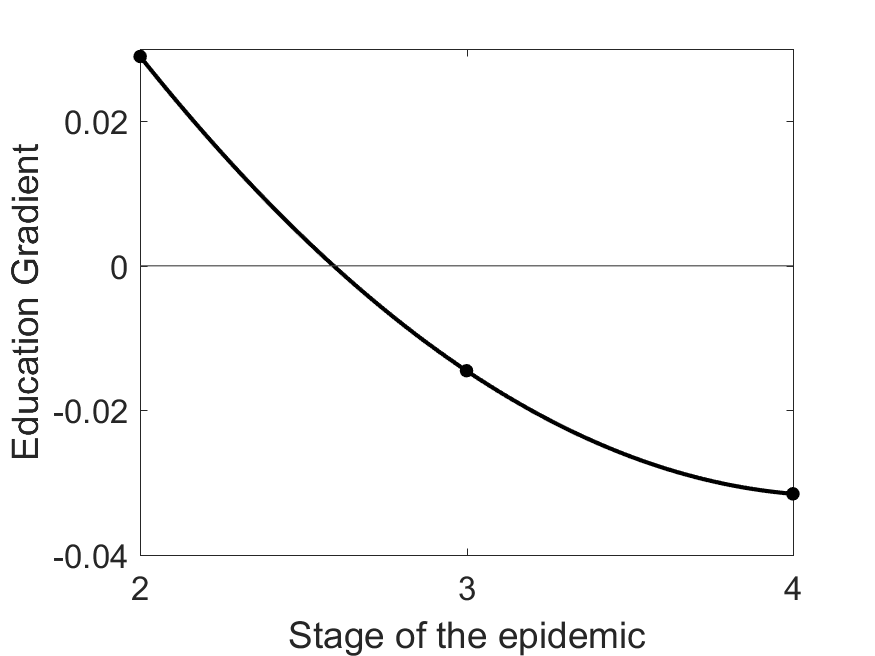
\includegraphics[width = 1\linewidth, height = 0.25\textheight]{figures/gradient/fig_grad1.png}
\label{fig_grad1}
\end{minipage}%
\begin{minipage}{.5\textwidth}
\centering
\captionof{figure}{HIV-education gradient\\ by gender}
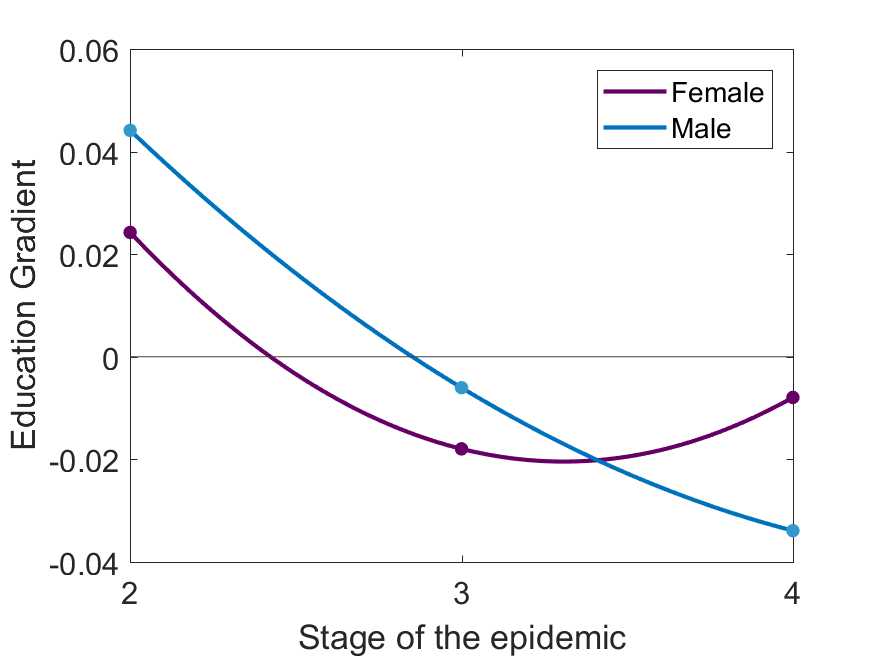
\includegraphics[width = 1\linewidth, height = 0.25\textheight]{figures/gradient/fig_grad2.png}
\label{fig_grad2}
\end{minipage}
\end{figure}

In order to understand the differences between educated risky sex buyers and risky sex producers, it is possible to conduct a simple sensitivity analysis on the estimation results. One way to increase the overall prevalence in the country is to increase labor income given to all individuals, in particular, any individual regardless if she/he is infected or not, will increase its chosen level of extramarital risky sex no matter what because of the income effect, as a result, overall prevalence among the population will increase. A second channel that increases prevalence among the educated buyers or producers is a reduction of the "comprehension parameter" $\rho_{e}$, since educated agents are less aware then they consume more risky sex. However these channels don't tell us anything about the prevalence by gender. On the other hand, there is a set endogenous outcomes generated by the sex market behavior and the amount of risky sex demanded by educated/uneducated sex buyers. In principle, if the price of risky sex increases, the total demand will decrease, how ever total demand might is still covered be covered in the same proportion by educated/uneducated risky sex producers. If demand for risky sex among uneducated sex buyers increases, it might be the case that prevalence among educated women increases since they also have to cover the increasing demand. In other words the market protects educated sex buyers, since in no way they will be forced to increase their sex consumption, but if uneducated buyers increase demand, both uneducated and educated producers must intervene to clear the sex market.    
%\section{Conclusions}\label{sec7}
In this paper I propose a general equilibrium heterogeneous agent model intended to help understand the dynamic relation between education and HIV diffusion. The model features two types of agents that differ primarily in their level of education, asset holdings and HIV status. The model identifies four stages of the HIV-epidemic: 1.A \textit{pre-epidemic stage}, where there is no risk of infection. 2. A \textit{myopic stage} where individuals do not realize the hazard of HIV infection and don't take it into account for consumption decisions. 3.A \textit{maturity stage} where individuals acknowledge the risk of infection and immediately adjust their expectations and consumption decisions. It is because of this reason that the equilibrium amount of extramarital risky sex in the maturity of the epidemic is less than that the \textit{myopic stage}. Finally the \textit{ARTs stage} introduces antiretroviral treatment that might cause the prevalence among educated people to increase. This can be explained by the fact that since educated individuals believe they have a lower risk of infection, then they start to increase their levels of extramarital risky sex again and this has overall positive effect on prevalences. \\

 The paper proposes an innovative algorithm that links all four epidemic stages together in order to have a dynamic representation of the HIV epidemic. The model is then calibrated for Malawi using mostly DHS data. Once the model is solved, I use the data generated by the model to calculate the HIV education gradient for Malawi and its dis aggregation by gender.\\
 
 The gradient has an evident U shape, however, after the \textit{myopic stage} the gradient becomes significantly negative, meaning that it is recommendable to increase the level of education of the population in order to reduce the risk of HIV infection. Moreover when looking at the gender dis-aggregation we note that education indeed reduces the probability of infection both  among men and women. But for the case of women after the \textit{maturity of the epidemic}, the education gradient starts to get closer to zero. This suggests that increasing the level of education of the female population in Malawi will not reduce HIV prevalence as in the \textit{maturity of the epidemic}. Quantitatively speaking, during the \textit{myopic stage}of the epidemic additional education increases the probability of infection by 2.9${\%}$ among the total population and among males and females 4.41${\%}$ and 2.42 ${\%}$ respectively. However during the \textit{ARTs stage} education actually reduces the risk of infection by  3.16${\%}$ among the total population and among men and women 3.39${\%}$ and 0.79 ${\%}$ respectively. 

\section{The model}\label{sec4}
\subsection{Model characteristics}
The model features two types agents: sex consumers and sex producers. They are finitely lived, have rational expectations and intend to maximize future discounted utility, $E_{0}\sum_{t}^{\infty}\beta^{t}u$, subject to their respective budget constraints. I assume the function $u:[0,\infty)\to \mathbb{R}$ is strictly increasing, strictly concave and twice continuously differentiable and has a CRRA form\footnote{$u(c)=\nicefrac{c^{1-\sigma}}{(1-\sigma)}$ for sex producers and $u(c,x)=\nicefrac{c^{1-\sigma}}{(1-\sigma)}+\nicefrac{x^{1-\sigma}}{(1-\sigma)}$ for sex buyers.  Note that all agents regardless of their type share the same relative risk aversion. }, with relative risk aversion parameter $\sigma>0$.

 Agents interact in three competitive markets in this economy: The goods market, the sex market and the assets market.  
\begin{itemize}
\item There are two types of agents sex buyers ($g$) and sex producers ($-g$).  
\item From the goods market agents can obtain consumption good $c$ at price $p_{1}$\footnote{The price of the consumption will as numeraire, then $p_{1}=1$}. 
\item Non-marital risky sex $x$ is traded in the sex market for price $p_{2}=p$. Where variable $x$ is continuous.
\item Individuals can either save or borrow in the asset market by trading a non-contingent asset $a$ with endogenous return $r$.
\item Agents education can either be high or low $e=\{1,0\}$.
\item HIV status can be positive or negative $h=\{1,0\}$.
\item Labor is supplied in elastically.
\item Agents receive labor income $y(e)$, where income differs according to their education level $e$. In particular $y(1)>y(0)$.
\item The model features an exogenous component of labor income $z$ that can take two values $z^{g}$ and $z^{b}$. $z$ captures stochastic income shocks in the economy and it follows a finite state Markov chain with a given transition matrix \textit{T}: 
\end{itemize}
\begin{align*}
    \pi(s'|s) = Prob(s_{t+1}=s'|s_{t}=s)=    \begin{bmatrix}%
    p_{gg} & p_{gb}\\
    p_{bg} & p_{bb}
    \end{bmatrix}
\end{align*}
\begin{itemize}
\item Let $\gamma_{e}$ denote the survival probability of an agent with level of education $e$.
\item Let $\psi^{h}_{e}$ be the fertility rate of an individual with HIV status $h$ and education $e$.
\item Let $\lambda(x,h)$ denote the probability of getting infected with HIV. Note that the probability of infection is actually a function of the amount of risky sex ($x$) consumed by the agent. This value is determined endogenously.
\end{itemize}
Following the discussion in Section\ref{sec1}, the model intends to characterize the different stages of the HIV epidemic according to the level of education of the population. In particular, the increase in the probability of infection for the most educated in the early and final stages.\\
In line with \cite{raul}, four stages of the epidemic have been identified. 
\begin{enumerate}
\item Pre-Epidemic stage
\item Miopic stage of the epidemic
\item Difussion and maturity of the epidemic
\item Introduction of anti-retro viral drugs
\end{enumerate}
\begin{comment}
The features of each stage will be described in detail in the upcoming sections.\\

The model features additional dynamics, in the sense that it intends to capture the evolution of the HIV epidemic starting from stage one until stage four. For presentation purposes each stage characterizes a stationary equilibrium, but later on they will be linked with the intention to describe the complete evolution of the HIV epidemic.
\end{comment}


In the following sections I describe in detail the characteristics of each of the stages of the model.  

\subsection{Pre-epidemic stage}\label{pre}
There is no probability of infection, namely $\lambda(x,h)=0$ and $\psi_{e}^{h=1}=\psi_{e}^{h=0}=\psi_{e}$. Agents differ on their type $g$, assets $a$ and education level $e$.\\

\noindent\textbf{Sex Buyers:}\\
For agents of type $g$ the dynamic problem is:
\begin{align}
V(a,e,g,s;\Phi) &= \mathop{\max_{c\geq 0,x \geq 0,a' \geq 0}}  u(c,x) + \beta \gamma_{e} \sum_{s'|s}\pi(s'|s)V(a',e,g,s';\Phi') \label{eq1}\\
\mbox{s.t}\nonumber\\
c+ px +a'&= zy(e) + (1+r(\Phi))a \label{eq2}\\
a' &\leq b
\end{align}

 Agents buys non-marital risky sex $x$ at price $p$ and save or borrow $a'$ with return $r$. Agents cannot borrow amounts that exceed $b$. Note that labor is supplied in elastically and depends on their level of education $e$, then their labor income is $y(e)$, where $y(1)>y(0)$.\\
 This problem is characterized by three individual state variables ($a,e,g,s$) and one aggregate state variable $\Phi$, which represents the population distribution over the states $a,e,g,s$. The choice variables are $c,x$ and $a'$.\\
\begin{comment}
 The above problem can be written in sequential form: 
\begin{align*}
\mathop{\max_{c_{t},x_{t},a_{t+1}}}&E_{0}\sum^{\infty}_{t=0}\beta^{t}u(c_{t},x_{t})  \\
\mbox{s.t}\\ 
c_{t}+p_{t}x_{t}+a_{t+1}&=y(e)+(1+r_{t})a_{t}
\end{align*}
 \textbf{FOC's:}\\
 \begin{align*}
 \frac{\partial u(c_{t},x_{t})}{\partial x_{t}}&=-u'_{c}(c_{t},x_{t})p_{t}+u'_{x}(c_{t},x_{t})=0\\
 \frac{\partial u(c_{t},x_{t})}{\partial a_{t+1}}&=-u'_{c}(c_{t},x_{t})+u'_{c}(c_{t+1},x_{t+1})(1+r_{t})\beta=0
 \end{align*}
 Given the price system $\{p_{t}\}_{t=0}^{\infty},\{r_{t}\}_{t=0}^{\infty}$ the solution is characterized by the sequence of allocations $\{c_{t}\}_{t=0}^{\infty}, \{x_{t}\}_{t=0}^{\infty}, \{a_{t}\}_{t=0}^{\infty}$ such that they solve the above maximization problem.\\
\end{comment}

\noindent \textbf{Sex Producers:}\\
For agents of type $-g$ the dynamic problem is:
\begin{align}
V(a,e,-g,s;\Phi) &= \mathop{\max_{c\geq 0, 1\geq l\geq 0,a' \geq 0}}  u(c) + \beta \gamma_{e} \sum_{s'|s}\pi(s'|s)V(a',e,-g,s';\Phi') \label{eq3}\\
\mbox{s.t}\nonumber\\
c +a'&= pl^{\alpha}+zy(e)(1-l) + (1+r(\Phi))a \label{eq4}\\
a' &\leq b
\end{align}
Note that for these agents, extra marital risky sex ($x$) does not generate any utility, then the utility function only depends on the amount of consumed ($c$). Additionally, these agents produce sex with a decreasing return to scale production function $x=l^{\alpha}$ where $\alpha\in(0,1)$. In other words, these agents produce non-marital risky-sex $x$ using time $l$ and sell it a price $p$. Where $l$ is the fraction of labor dedicated to the production of extramarital risky sex, the remaining labor ($1-l$), which is not allocated to sex production, is sold in the market for labor income $y(e)$. As before, agents are allowed to save or borrow assets $a$ at rate $r$.\\

\begin{comment}
\noindent The above problem can be written in sequential form: 
\begin{align*}
\mathop{\max_{c_{t},l_{t},a_{t+1}}}&E_{0}\sum^{\infty}_{t=0}\beta^{t}u(c_{t})  \\
\mbox{s.t}\\ 
c_{t}+a_{t+1}&=p_{t}l_{t}^{\alpha}+y(e)(1-l_{t})+(1+r_{t})a_{t}
\end{align*}
 \textbf{FOC's:}\\
 \begin{align*}
 \frac{\partial u(c_{t})}{\partial l_{t}}&=-u'_{c}(c_{t})(\alpha p_{t} u^{\alpha-1}-y(e))=0\\
 \frac{\partial u(c_{t})}{\partial a_{t+1}}&=-u'_{c}(c_{t})+u'_{c}(c_{t+1})(1+r_{t})\beta=0
 \end{align*}
 Given the sequence of prices $\{p_{t}\}_{t=0}^{\infty},\{r_{t}\}_{t=0}^{\infty}$ the solution are the sequences of allocations $\{c_{t}\}_{t=0}^{\infty},\{l_{t}\}_{t=0}^{\infty}, \{l_{t}\}_{t=0}^{\infty}, \{a_{t}\}_{t=0}^{\infty}$ that solve  the agent's problem.\\
 
\end{comment}


 \subsection*{The aggregate state variable and transition function}
\noindent The aggregate state variable evolves according to:
\begin{align}
\Phi'=F(\Phi)
\end{align} 
Where the function $F:\mathcal{M}\to\mathcal{M}$ is the aggregate law of motion, mapping distributions to distributions. $F$ summarizes how agents move within the distribution of assets , education and type from one period to the next, however this is exactly what a transition function tell us. \\
\noindent Define the transition function $\mathcal{Q}:\mathcal{Z}\times\mathcal{B(Z)}\to[0,1]$ by: 
\begin{align*}
Q((a,e,g,s)(\mathcal{A},\mathcal{E},\mathcal{G},\mathcal{S})) &= \left\{
\begin{tabular}{clc}
$\gamma_{e}$ & if      & $a(a,e,g,s;\Phi) \in \mathcal{A} $\\
0 & else & 
\end{tabular}
\right.\\
\forall \,\,\,(a,e,g,s)&\in\mathcal{Z}\,\,\,\mbox{and}\,\,\,(\mathcal{A,E,G,S})\in{\mathcal{B(Z)}}
\end{align*}
Where $\mathcal{Z}$ consists of all n-tuples of $A\times E\times G\times S$. \\
Define $\mathcal{B(Z)}$ as the set of Borel sets on $\mathcal{Z}$, in particular $\mathcal{A,E,G,S}\in\mathcal{B(Z)}$ where $\mathcal{A,E,G,S}$ are projections of $\mathcal{Z}$ over the spaces $A,E,G$ and $S$ respectively. Let $\mathcal{P}$ be a probability measure on $\mathcal{B(Z)}$, then $\mathcal{P}: \mathcal{B(Z)}\to[0,1]$.\\
Then the evolution of the asset distribution is:
\begin{align}
\Phi'(\mathcal{A,E,G,S}) = F(\Phi) (\mathcal{A,E,G,S})= \int_{a,e,g,s} Q((a,e,g,s)(\mathcal{A,E,G,S})) d \Phi\\+\psi_{e}\Phi((a',e,g,s')(\mathcal{A,E,G,S}))
\end{align}
Which is the fraction of people with assets in $\mathcal{A}$, education $\mathcal{E}$, type $\mathcal{G}$ and states in $\mathcal{S}$ as measured by $\Phi$, that transit to ($\mathcal{A,E,G,S}$) as measured by $\mathcal{Q}$. The last term accounts for the new born. Population of each group increases according to their respective fertility rate $\psi_{e}$. It important to note that individuals of a certain type give birth to people of the same type.
 \subsection*{Solution to the recursive problem}
 Given prices $p,r$ the solution to the recursive problem of agents $g$ and $-g$  are the policy functions $a'(a,e,g,s;\Phi), x(a,e,g,s;\Phi), c(a,e,g,s;\Phi), l(a,e,g;\Phi)$ that induce a stationary distribution $\Phi(\mathcal{A,E,G,S})$ over the set of state variables. Where $\Phi$ is the aggregate state variable.
 \subsection*{Stationary equilibrium}
 The \textit{stationary equilibrium of the Pre-Epicemic stage} is:
 \begin{itemize}
 \item An interest rate $r$ and price $p$
 \item Policy functions $a'(a,e,g,s;\Phi), x(a,e,g,s;\Phi), c(a,e,g,s;\Phi), l(a,e,g,s;\Phi)$
 \item A stationary distribution $\Phi(\mathcal{A,E,G,S}) $
 \end{itemize}
 Such that:
 \begin{enumerate}[label=\alph*]
 \item Given $r$ and $p$ the policy functions  $a'(a,e,g,s;\Phi), x(a,e,g,s;\Phi), c(a,e,g,s;\Phi), l(a,e,g,s;\Phi)$ solve the sex buyers and sex producers problem respectively. 
 \item The stationary probability distribution $\Phi'(\mathcal{A,E,G,S})$ is induced by the optimal policy $a'(a,e,g,s;\Phi)$.
 \item All markets clear. 
  \end{enumerate}
 \begin{align*}
\int_{a,e,g,s} a'(a,e,g,s;\Phi) d\Phi &= 0 \\
\int_{a,e,g,s} x(a,e,g,s;\Phi) d \Phi &= \int_{a,e,-g,s} x(a,e,-g,s;\Phi) d\Phi
\end{align*} 
That is, there is zero net supply of assets, the sex markets clear and the consumption market clears by Walras law. 
\subsection*{Computing the stationary equilibrium for the Pre-epidemic stage}
\noindent \textbf{Calibration of the parameters:}\\
\begin{center}
\begin{longtable}{ccc}
\caption{List of parameters}\\%
\hline%
\multicolumn{1}{c}{\textbf{\LaTeX}} &
\multicolumn{1}{c}{\textbf{Description}} &
\multicolumn{1}{c}{\textbf{Value}}\\%
\hline\hline%
\endfirsthead
\multicolumn{3}{c}{{\tablename} \thetable{} -- Continued}\\%
\hline%
\multicolumn{1}{c}{\textbf{\LaTeX}} &
\multicolumn{1}{c}{\textbf{Description}}\\%
\hline\hline%
\endhead
${\beta}$ & Discount factor & 0.99\\
${\alpha}$ & Labor share of income & 0.1\\
${\sigma}$ & Risk aversion & 1.5 \\
${\gamma_{e=1}}$ & Survival rate educated (\%) & 99\\
${\gamma_{e=0}}$ & Survival rate less educated (\%) & 98\\
${\psi_{e=1}}$ & Fertility rate educated (\%) & 3\\
${\psi_{e=0}}$ & Fertility rate less educated (\%) & 6\\
${\omega}$ & People with at least secondary education (\%) & 32\\
${y_{e=1,t}}$ & Endowment educated at period $t$ & 0.75\\
${y_{e=0,t}}$ & Endowment less educated at period $t$ & 0.56\\
$s^{g}$ & Positive income shock & 1.06\\
$s^{b}$ & Negative income shock & 0.94\\
$p_{gg}$ & Transit probability from $z_{g}$ to $z_{g}$ & 0.95\\
$p_{gb}$ & Transit probability from $z_{g}$ to $z_{b}$ & 0.05\\
$p_{bg}$ & Transit probability from $z_{b}$ to $z_{g}$ & 0.05\\
$p_{bb}$ & Transit probability from $z_{b}$ to $z_{b}$ & 0.95\\
$a_{min}$ & Lower limit of the asset grid & -5 \\
$a_{max}$ & Upper limit of the asset grid & 8\\
$n$ & number of nodes in the asset grid& 7\\

\hline%
\end{longtable}
\end{center}

The values for $\beta, \alpha, \sigma$ are standard in the literature. The survival rate $\gamma_{e}$ and fertility rate were $\psi$ are data form the World Bank, Sustainable Development Indicators for Malawi. Additionally the share of people with at least secondary education has been taken from DHS\footnote{Demographic and health survey} data for Malawi.\\

$b$ is set to be the models natural borrowing constrain, this means that agents do not have any kind of liquidity constraint as in the pre-epidemic stage the natural borrowing constraint is never binding. Additionally $a_{min}$ has been chosen low enough to surpass the natural borrowing constraint $b$ set by the model. Consequently $a_{max}$ has been chosen large enough so that agents do not hold assets in excess of $a_{max}$ in the stationary equilibrium. The choice of $n$ is arbitrary, higher numbers of $n$ incur in longer computing time.

\noindent \textbf{\textit{Algorithm No.1}: Computation of the stationary equilibrium:}\\

\noindent\textit{Step 1: Make initial guesses of price $p$ and interest rate $r$.\\
Step 2: Compute the agents decision rules.\\
Step 3: Compute the stationary distribution of assets (follow Algorithm No.2).\\
Step 4: Compute aggregate assets demand and aggregate sex demand. Check the aggregate consistency conditions.\\
Step 5: If conditions are not met, update $p$ and $r$ and return to Step 2. 
}\\

Keep in mind that \textit{Algorithm No.1} is generic enough so that it can also be applied to compute the stationary equilibrium of any stage of the HIV epidemic.\\

For the computation of the decision rules I make use of value function iteration with linear interpolation as described in any computational methods text book\footnote{Refer to \cite{mauss}, \cite{judd}, \cite{sargent}}. For the value function iteration procedure it is necessary to choose a grid over the asset space $A=\{a_{1}=a_{min},...,a_{n}=a_{max}\}$ where $a_{min}$ and $a_{max}$ are the values chosen in the calibration. \\

\noindent\textbf{\textit{Algorithm No.2}: Computation of the invariant distribution:}\\

\noindent\textit{Step 1: Choose a grid over the asset space $A=\{a_{1}=a_{min},...,a_{n}=a_{max}\}$.\\
Step 2: Set a time iteration counter $t=0$ and choose an initial (discrete) density function $\phi_{0}(a,e,g,s)$ over the state space.\\
Step 3: Initialize $\phi_{t+1}(a',e,g,s')$\footnote{$\phi_{t+1}$ is of dimensions $n\times (m*w*q)$, where $m=2$, $w=2$ and $q=2$ since education, type and stochastic states can only be of two sorts.} and compute the optimal next period wealth $a'$ with the help of the decision rule.\\
Step 4: For all $a'\in A$, $e \in E$, $g \in G$ and $s \in S$compute the following expression:}
\begin{align}\label{eq:10}
    \phi_{t+1}(a',e,g,s')=\sum_{a,e,s}\sum_{s'|s}\textbf{1}_{a'\in\mathcal{A}}\gamma_{e}\pi(s'|s)\phi_{t}(a,e,g,s) + \psi_{e}\phi_{t}(a',e,g,s')
\end{align}
\textit{
Step 5: If $|\phi_{t+1}-\phi_{t}|<exp(-12)$ stop, otherwise set $\phi_{t}=\phi_{t+1}$ and return to Step 3.}\\

For simplicity reasons the grid chosen for \textit{Algorithm No.2} is the same as the grid chosen for the value function iteration procedure in \textit{Algorithm No.1}, otherwise if the grid would be finer it would be necessary to include the probabilities of $a'(a,e,g,s)$ falling between the respective points in the grid.\\

For \textit{Step2} of \textit{Algorithm No.2} I choose the uniform distribution as the initial values of the distribution. The algorithm should converge regardless of the choice of the initial distribution. 


%\subsection*{Computing the dynamics for the pre-epidemic stage}


\subsection*{Results}
\begin{table}[H]
\caption{Equilibrium prices}%
\begin{center}
\begin{tabular}{r|c}
\hline%
\textbf{Price of sex} &0.32\\
\hline
\textbf{Interest Rate} & 9.25\%\\
\hline%
\end{tabular}
\end{center}
\end{table}

%\begin{figure}[t!]

\begin{figure}[H]
\caption{Equilibrium}
\hspace{-2.0cm}
\begin{center}
\begin{tabular}{cc}
\multicolumn{1}{c}{(a) Sex Market} &  
\multicolumn{1}{c}{(b) Asset Market} \\
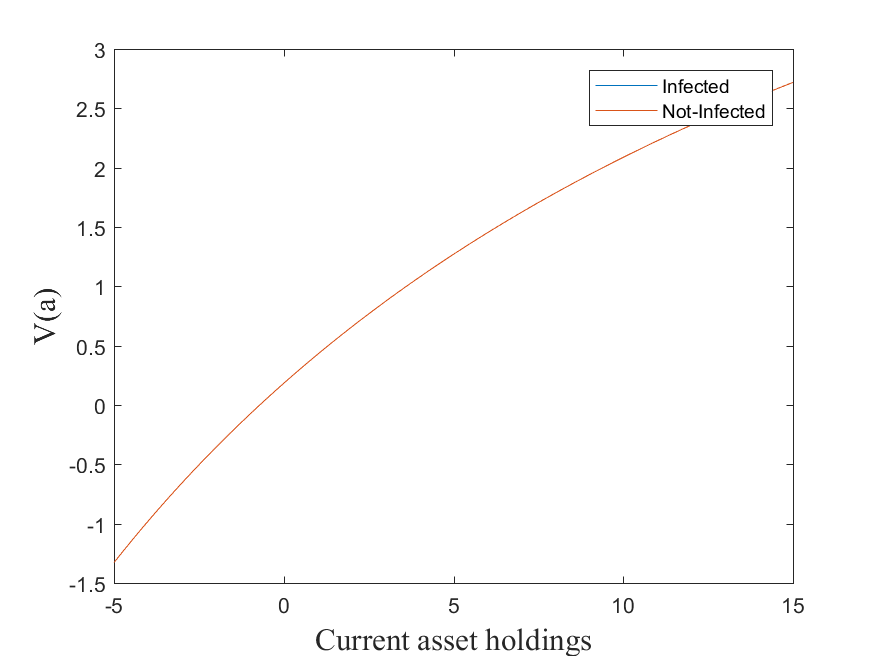
\includegraphics[angle=0,width=.5\textwidth]{figures/FIG14.png}   & 
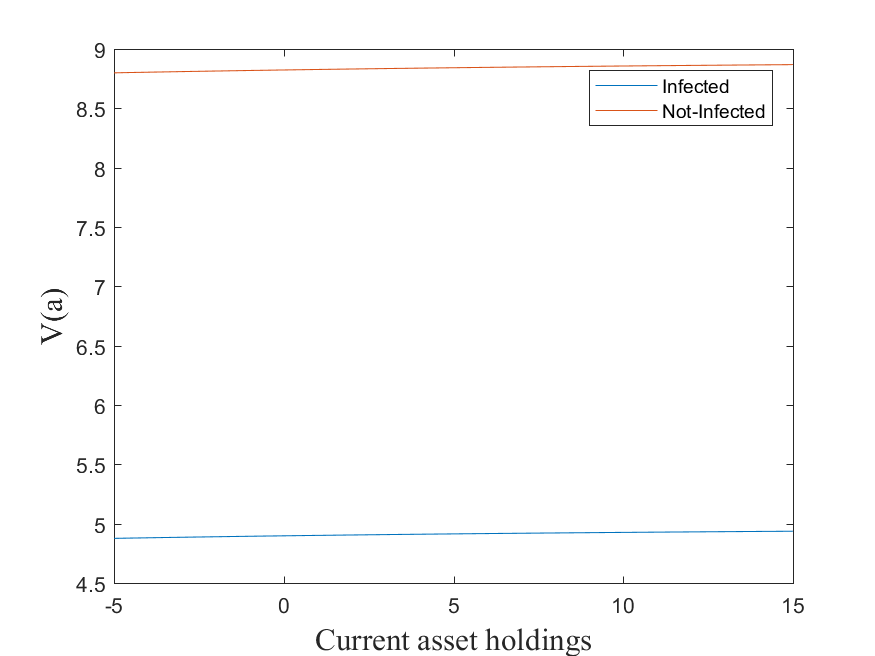
\includegraphics[angle=0,width=.5\textwidth]{figures/FIG15.png} 

%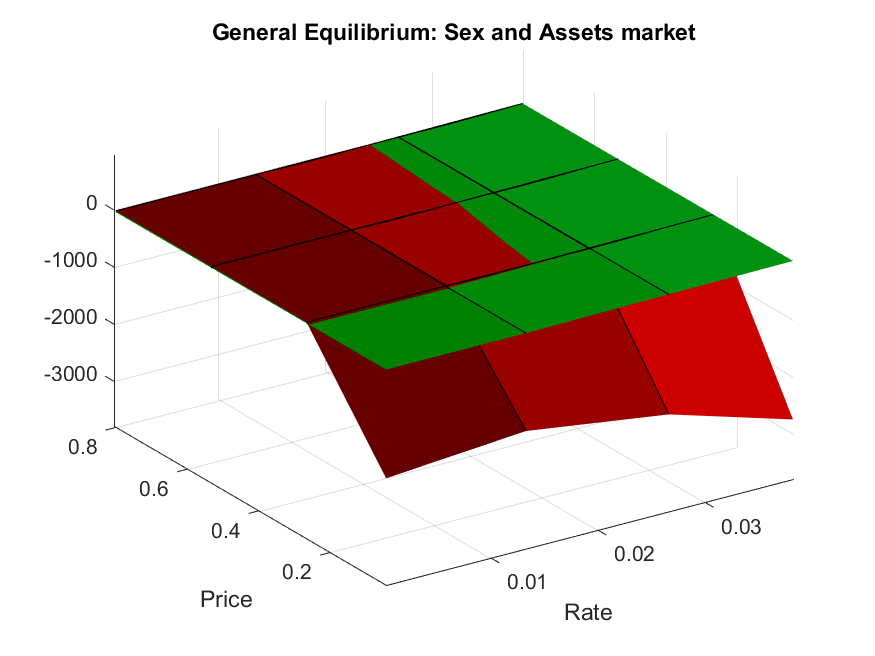
\includegraphics[angle=0,width=.5\textwidth]{figures/FIG_EQUILIBIUM3.png} 
\end{tabular}
\end{center}
\label{fig:6}
\end{figure}

\begin{figure}[H]
\caption{Distributions}
\hspace{-2.0cm}
\begin{center}
\begin{tabular}{cc}
\multicolumn{1}{c}{(a) Asset Distribution} &  
\multicolumn{1}{c}{(b) Income Distribution} \\
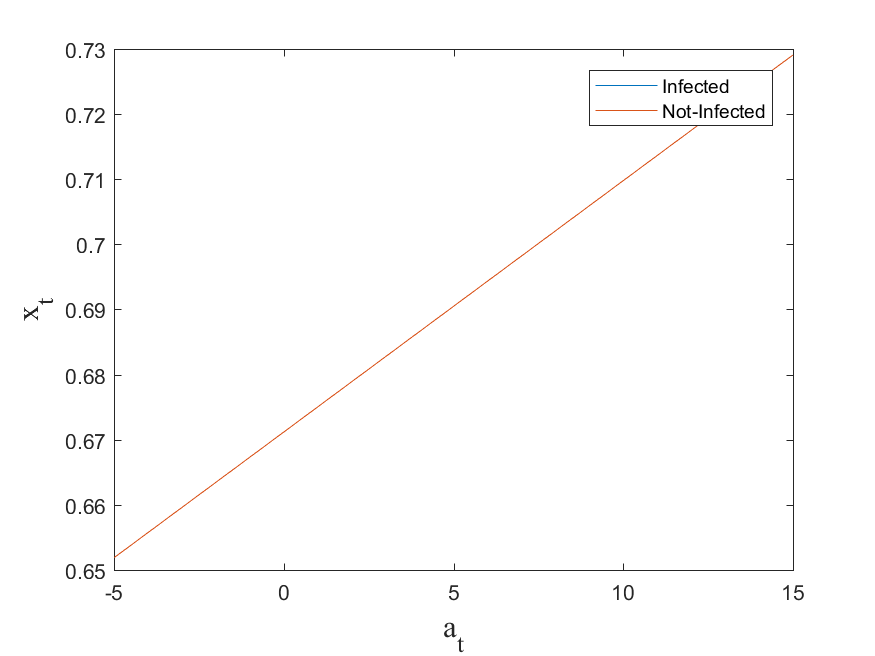
\includegraphics[angle=0,width=.5\textwidth]{figures/FIG9.png}   & 
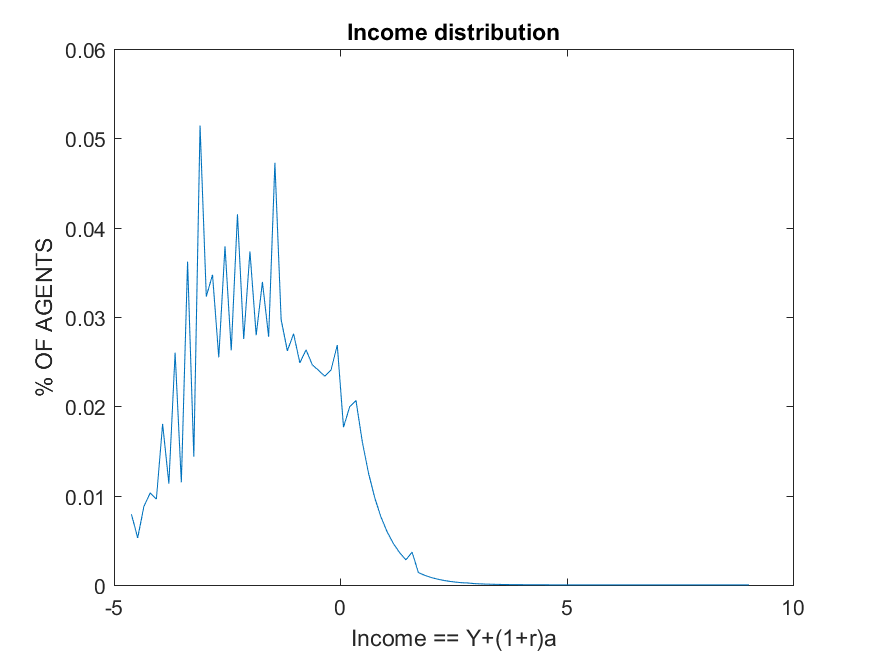
\includegraphics[angle=0,width=.5\textwidth]{figures/FIG10.png} 
\end{tabular}
\end{center}
\label{fig:4}
\end{figure}
\subsection{Miopic stage of the epidemic}
In this stage there exists a positive probability of getting HIV infected. $\lambda(x,h) >=0$. The particular characteristic of this stage is that the agents are not aware of the risk of infection, therefore they keep their sex consumption profile intact.\\
The probability of infection depends on the amount of sex consumed by the individuals following the following relation:
\begin{align}
    \lambda(x,0)=\frac{e^{x}}{e^{x}+\rho e^{-x}}
\end{align}
The infection transition matrix: 
\begin{align}
     \lambda(x,h'|h) = Prob(h_{t+1}=h'|h_{t}=h)=    \begin{bmatrix}%
    1-\lambda(x,0) & \lambda(x,0)\\
    \lambda(x,1)=0 & \lambda(x,1)=1
    \end{bmatrix}
\end{align}
Additionally, individuals that are HIV infected have a higher probability of dying and more educated individuals tend to consume have a lower probability of infection for no reason.\\
\textbf{Solving the Miopic stage}\\
The Miopic stage was solved by iterating forward over the policy rules obtained from the Pre-epidemic stage but keeping track of the evolution of the epidemic and demographics acording to Equation \ref{eq:10}\\
\textbf{Calibration of  the Miopic stage}\\
\begin{center}
\begin{longtable}{ccc}
\caption{List of parameters}\\%
\hline%
\multicolumn{1}{c}{\textbf{\LaTeX}} &
\multicolumn{1}{c}{\textbf{Description}} &
\multicolumn{1}{c}{\textbf{Value}}\\%
\hline\hline%
\endfirsthead
\multicolumn{3}{c}{{\tablename} \thetable{} -- Continued}\\%
\hline%
\multicolumn{1}{c}{\textbf{\LaTeX}} &
\multicolumn{1}{c}{\textbf{Description}}\\%
\hline\hline%
\endhead

${\gamma_{e=1,h=0}}$ & Survival rate educated healthy(\%) & 99.0\\
${\gamma_{e=0,h=0}}$ & Survival rate less educated healthy(\%) & 98.0\\
${\gamma_{e=1,h=1}}$ & Survival rate educated infected(\%) & 98.5\\
${\gamma_{e=0,h=1}}$ & Survival rate less educated infected(\%) & 97.5\\


\hline%
\end{longtable}
\end{center}
\textbf{Results}\\

\begin{figure}[H]
\caption{Evolution of the prevalence overtime}
\hspace{-2.0cm}
\begin{center}
\begin{tabular}{c}
\multicolumn{1}{c}{Evolution of the prevalence overtime} \\  
%\multicolumn{1}{c}{(b) Asset Market} \\
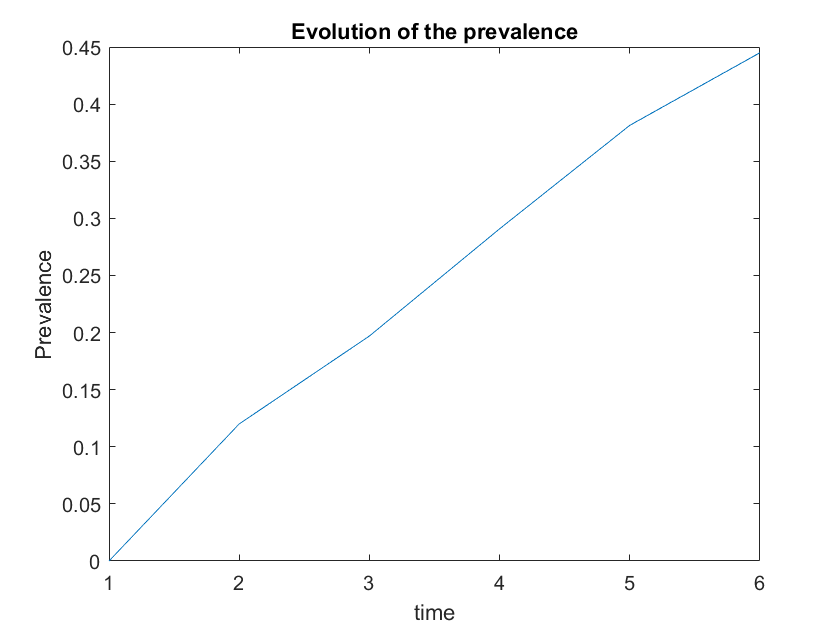
\includegraphics[angle=0,width=.5\textwidth]{figures/PREV.png}   
%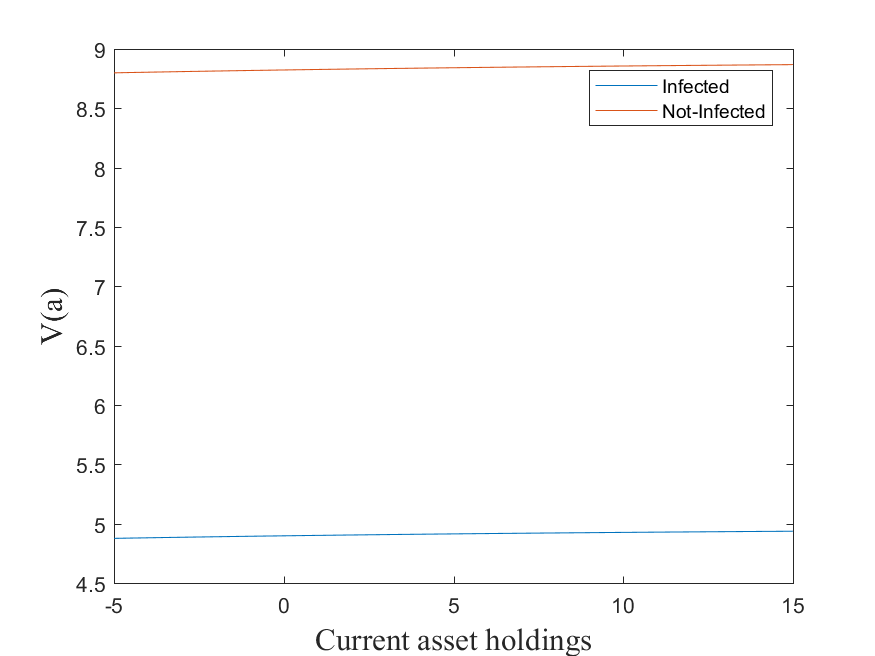
\includegraphics[angle=0,width=.5\textwidth]{figures/FIG15.png} 

%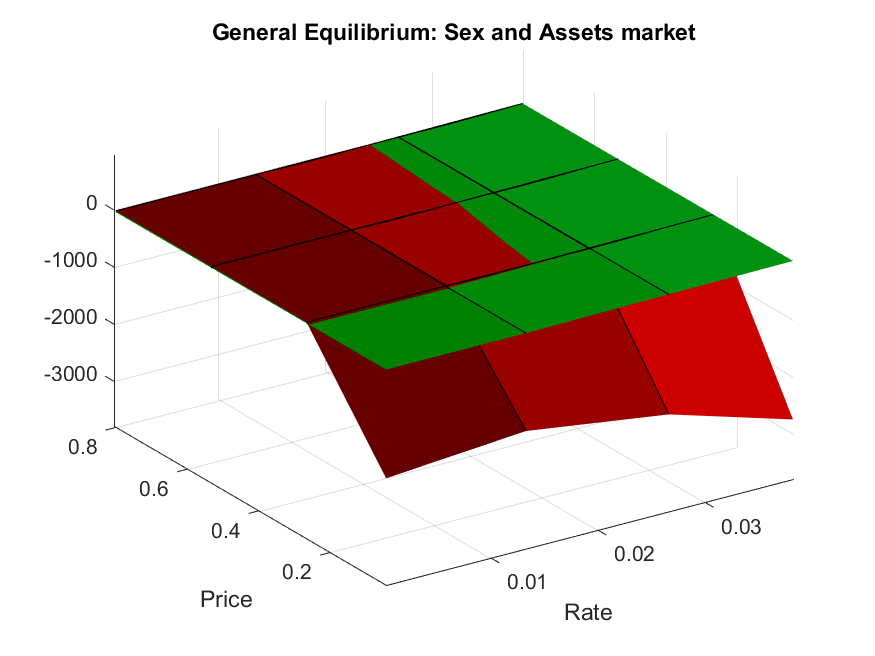
\includegraphics[angle=0,width=.5\textwidth]{figures/FIG_EQUILIBIUM3.png} 
\end{tabular}
\end{center}
\label{fig:6}
\end{figure}



\section{Aprendix}
\subsection{Pre-Epidemic graphs}
\begin{figure}[H]
\caption{Policy Functions Educated Buyers}
\hspace{-2.0cm}
\begin{center}
\begin{tabular}{cc}
\multicolumn{1}{c}{(a) Value function} &  
\multicolumn{1}{c}{(b) Assets function} \\
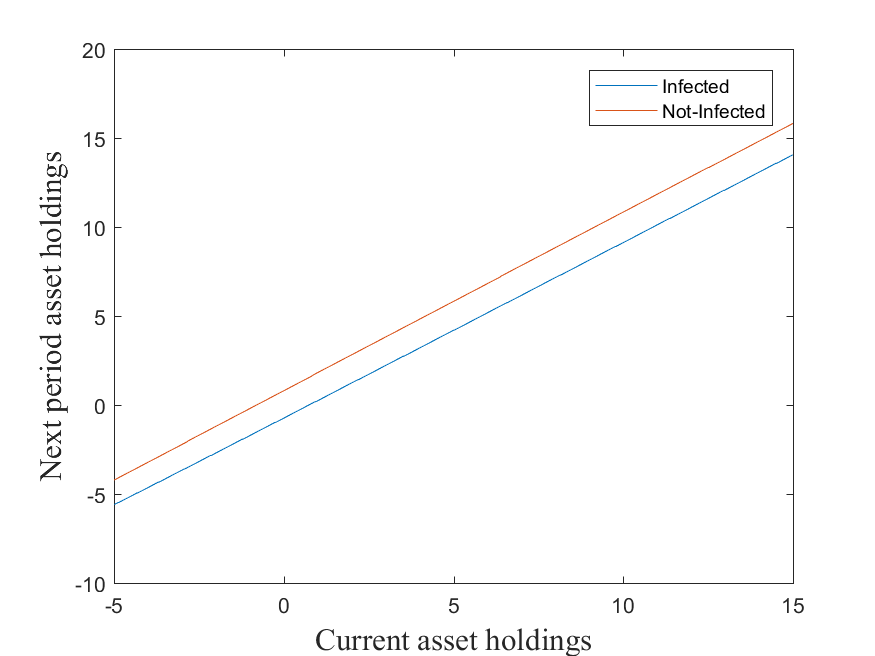
\includegraphics[angle=0,width=.5\textwidth]{figures/FIG1.png}   & 
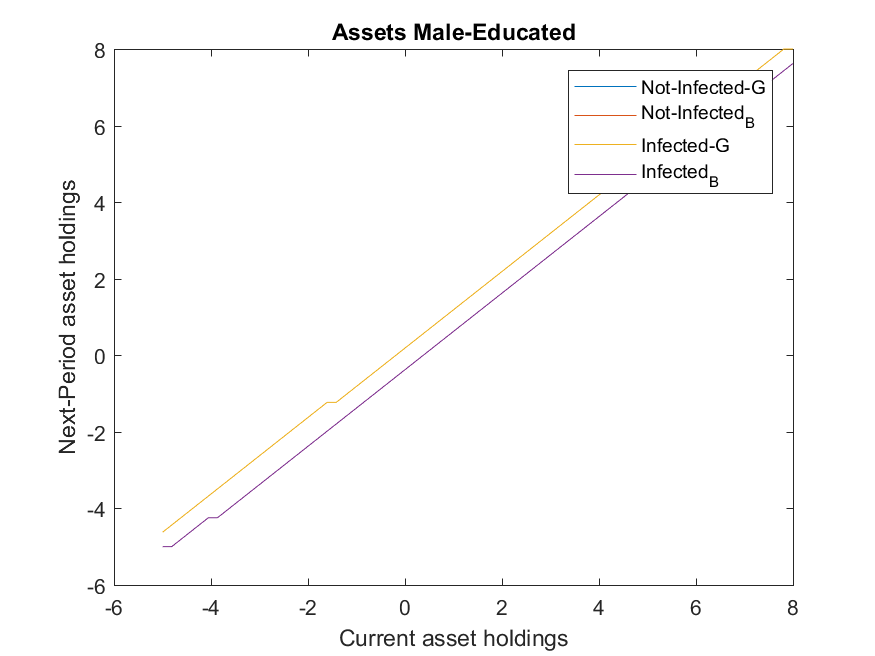
\includegraphics[angle=0,width=.5\textwidth]{figures/FIG3.png} \\
\multicolumn{1}{c}{(c) Consumption function} &  
\multicolumn{1}{c}{(d) Sex consumption function } \\
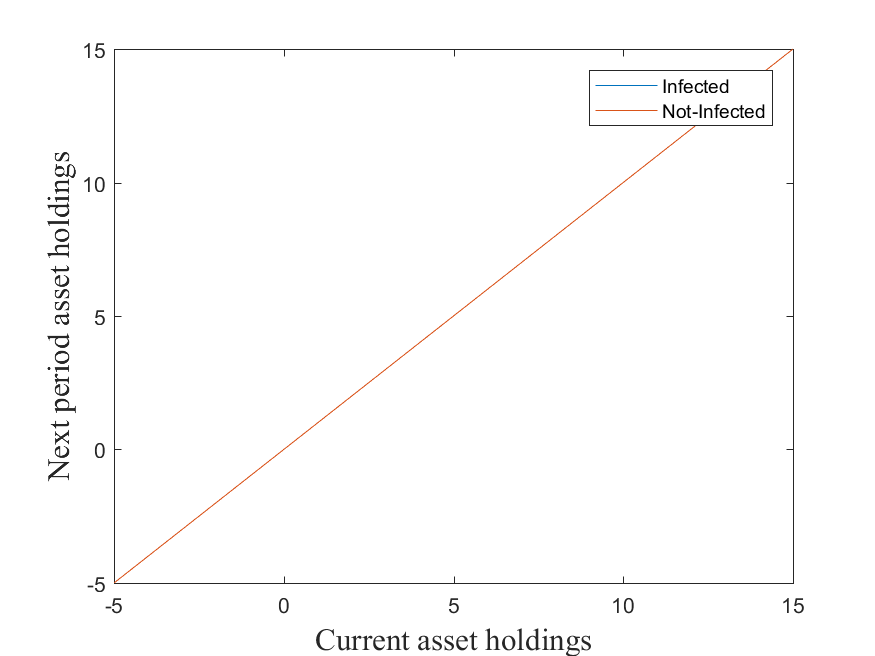
\includegraphics[angle=0,width=.5\textwidth]{figures/FIG2.png}   & 
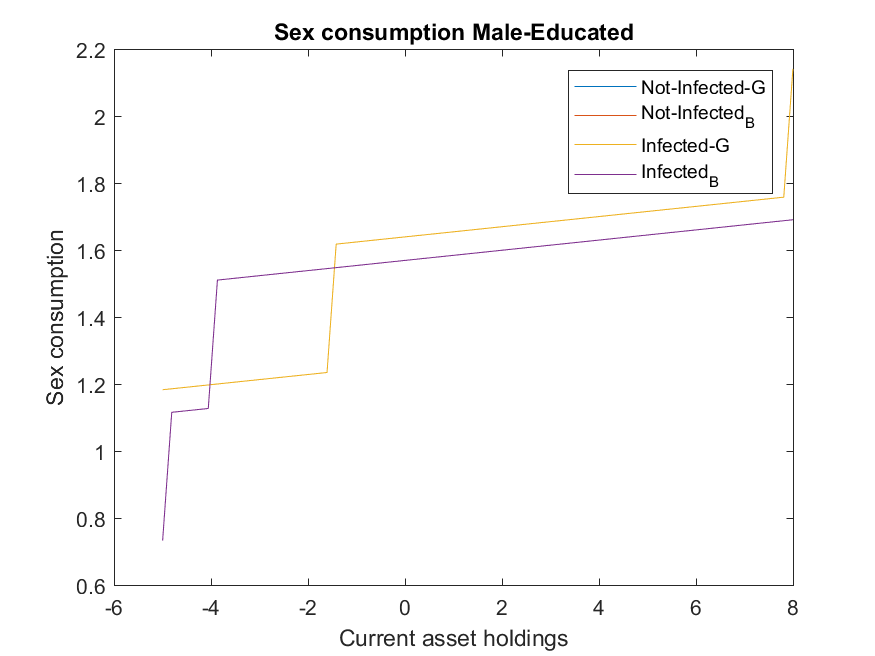
\includegraphics[angle=0,width=.5\textwidth]{figures/FIG4.png} \\
%\multicolumn{1}{c}{(a) Value function} &  
%\multicolumn{1}{c}{(b) Assets function} \\
\end{tabular}
\end{center}
\label{fig:2}
\end{figure}

\begin{figure}[H]
\caption{Policy Functions Educated Sellers}
\hspace{-2.0cm}
\begin{center}
\begin{tabular}{cc}
\multicolumn{1}{c}{(a) Value function} &  
\multicolumn{1}{c}{(b) Asset function} \\
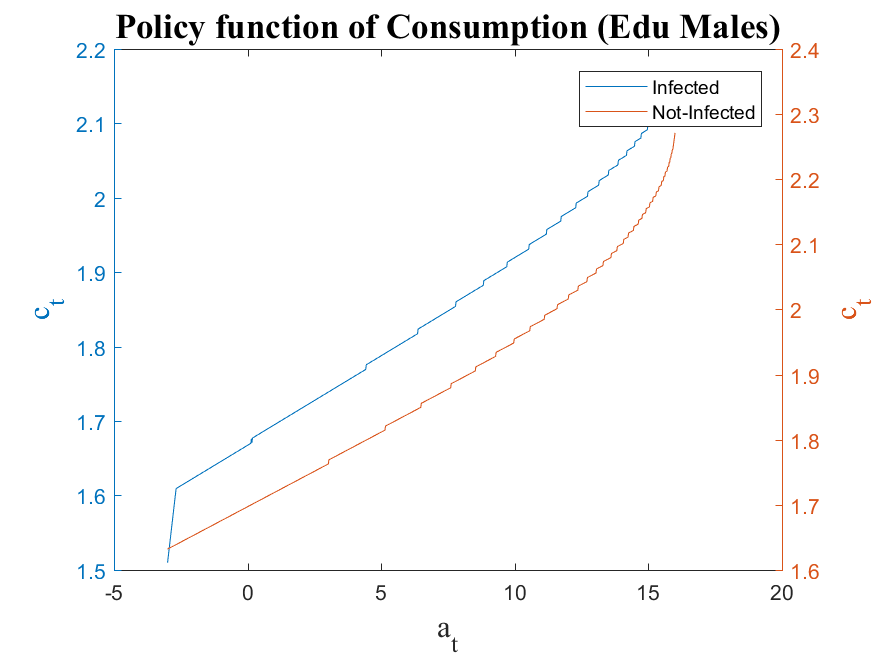
\includegraphics[angle=0,width=.5\textwidth]{figures/FIG5.png}   & 
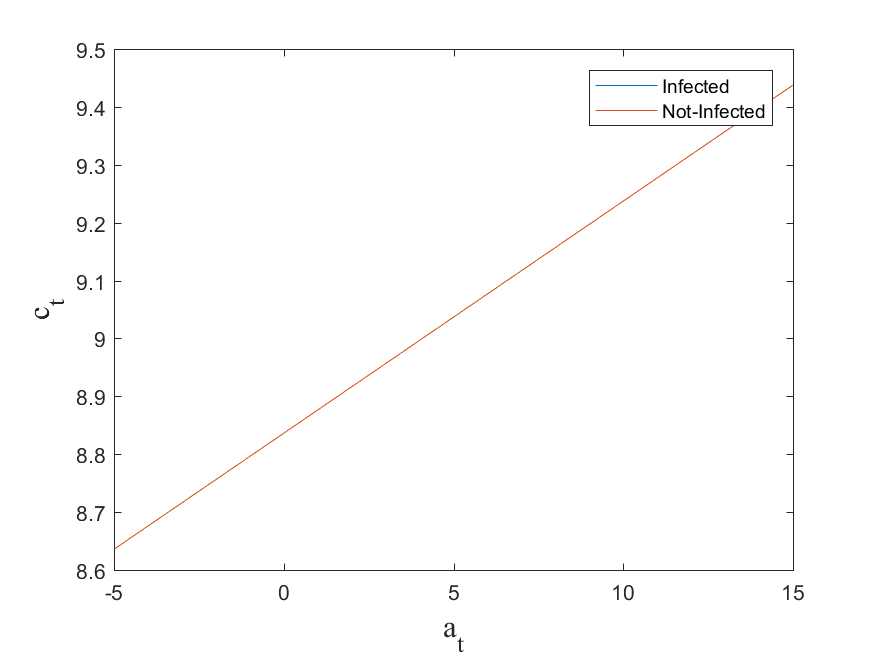
\includegraphics[angle=0,width=.5\textwidth]{figures/FIG7.png} \\
\multicolumn{1}{c}{(c) Consumption function} &  
\multicolumn{1}{c}{(d) Sex Production function } \\
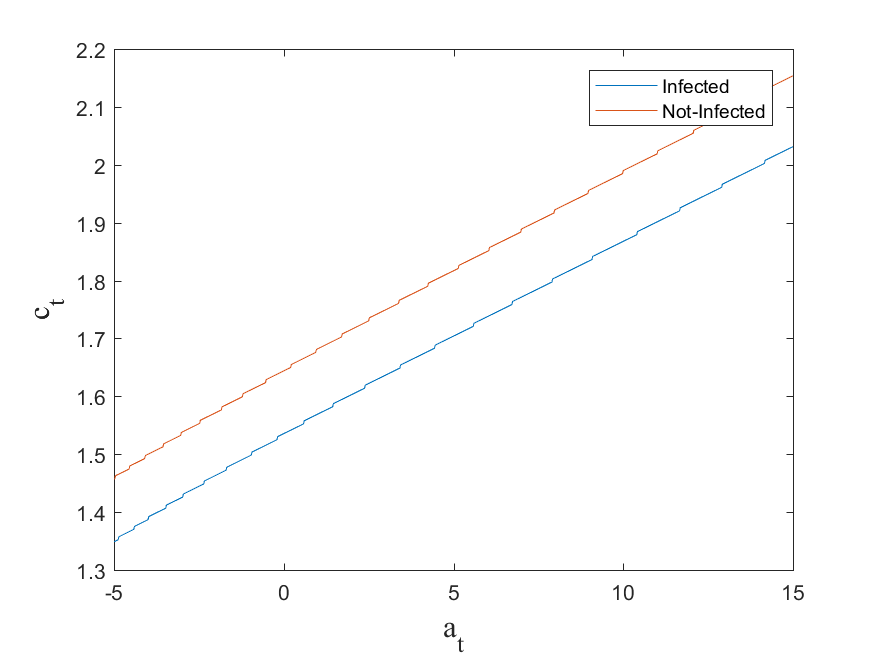
\includegraphics[angle=0,width=.5\textwidth]{figures/FIG6.png}   & 
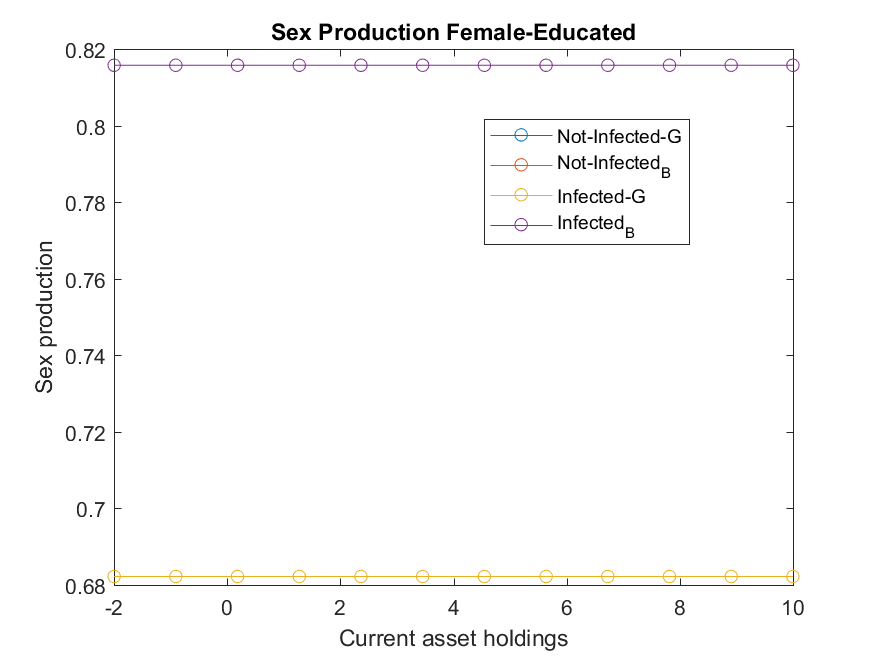
\includegraphics[angle=0,width=.5\textwidth]{figures/FIG8.png} \\
\end{tabular}
\end{center}
\label{fig:3}
\end{figure}



\begin{figure}[H]
\caption{Comparison plots}
\hspace{-2.0cm}
\begin{center}
\begin{tabular}{cc}
\multicolumn{1}{c}{(a) Asset Policy Functions} &  
\multicolumn{1}{c}{(b) Consumption Policy Functions} \\
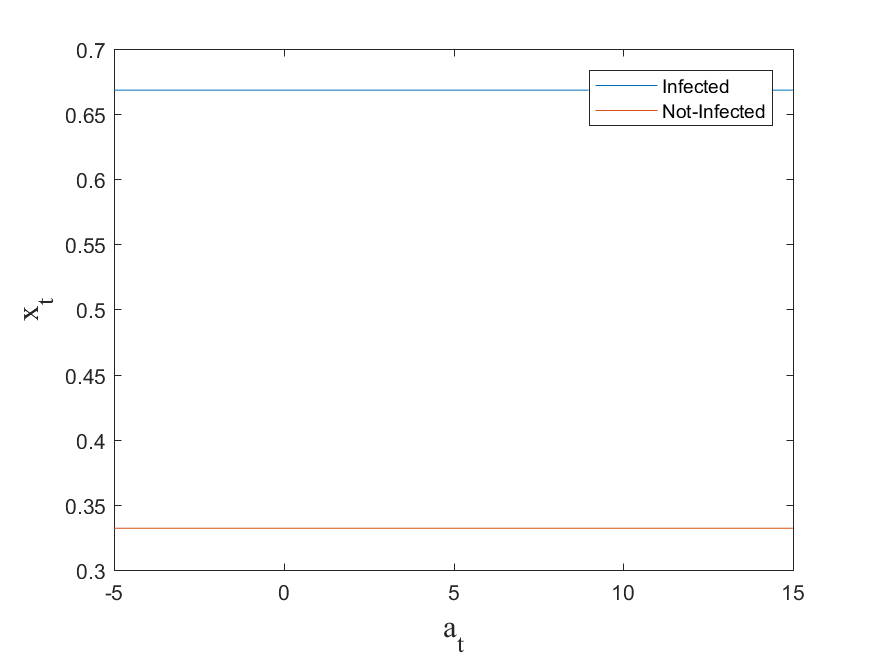
\includegraphics[angle=0,width=.5\textwidth]{figures/FIG11.png}   & 
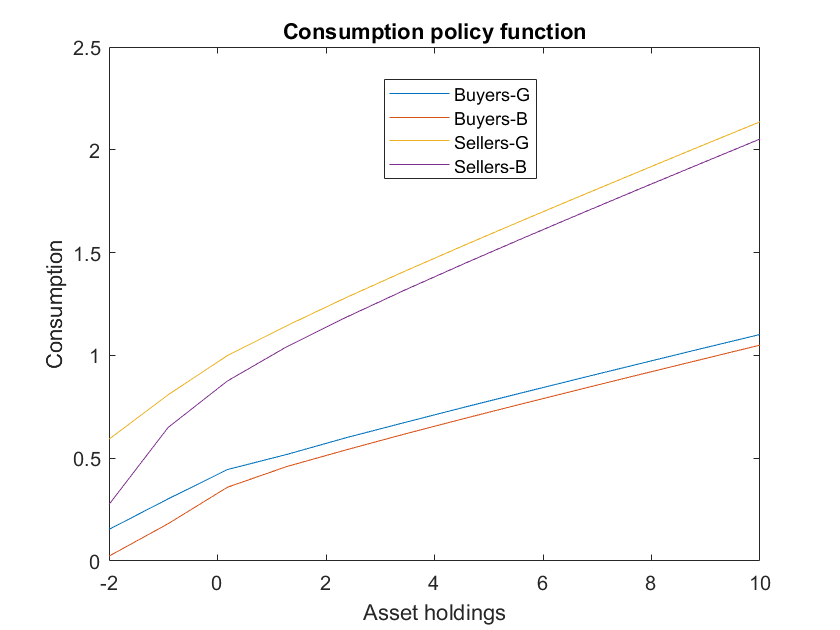
\includegraphics[angle=0,width=.5\textwidth]{figures/FIG12.png}\\ 
\multicolumn{2}{c}{(c) No Capital Income} \\  
%\multicolumn{2}{c}{(d) Equilibrium(repeated)} \\
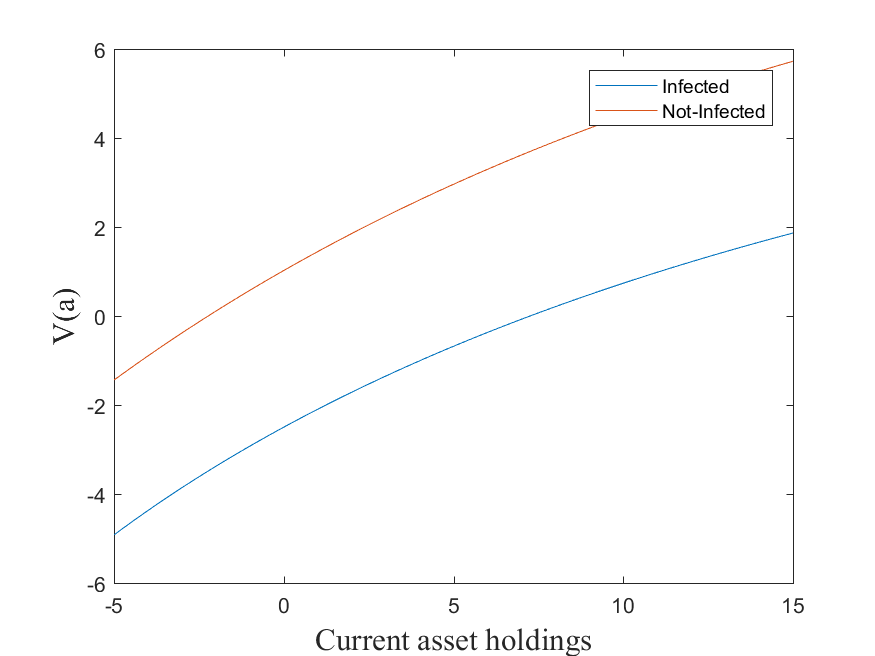
\includegraphics[angle=0,width=.5\textwidth]{figures/FIG13.png} 
%& 
%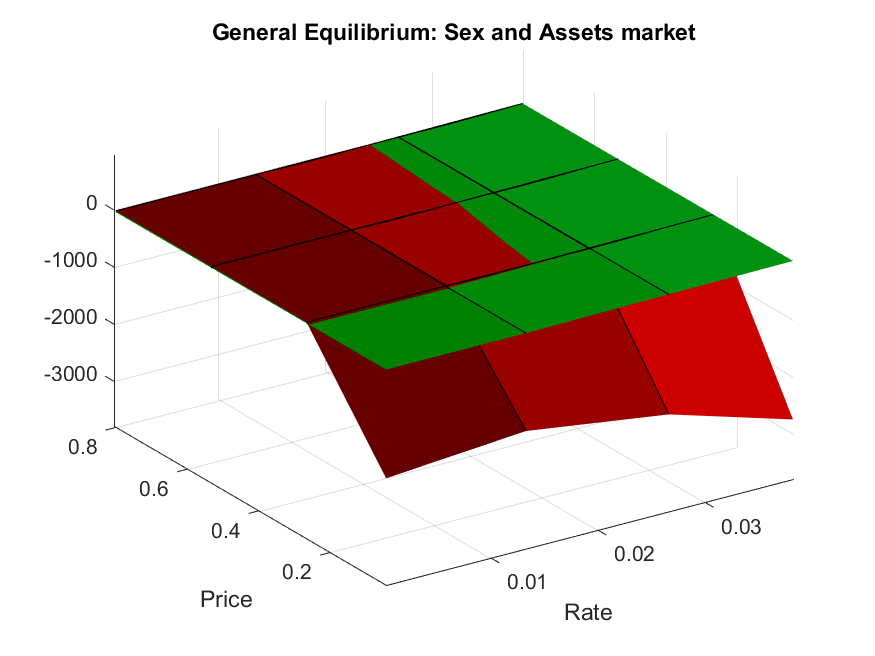
\includegraphics[angle=0,width=.5\textwidth]{figures/FIG_EQUILIBIUM3.png} 
\end{tabular}
\end{center}
\label{fig:5}
\end{figure}

\begin{figure}[H]
\caption{General equilibrium surface plots}
\hspace{-2.0cm}
\begin{center}
\begin{tabular}{cc}
\multicolumn{1}{c}{(a) Excess demand of Sex} &  
\multicolumn{1}{c}{(b) Excess demand of Assets} \\
%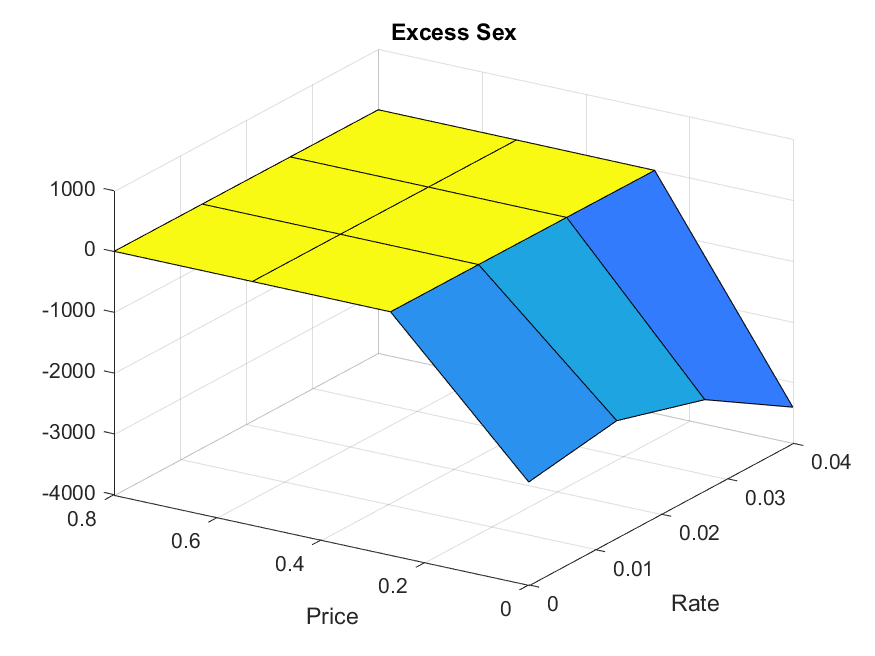
\includegraphics[angle=0,width=.5\textwidth]{figures/FIG_EQUILIBIUM2.png}   & 
%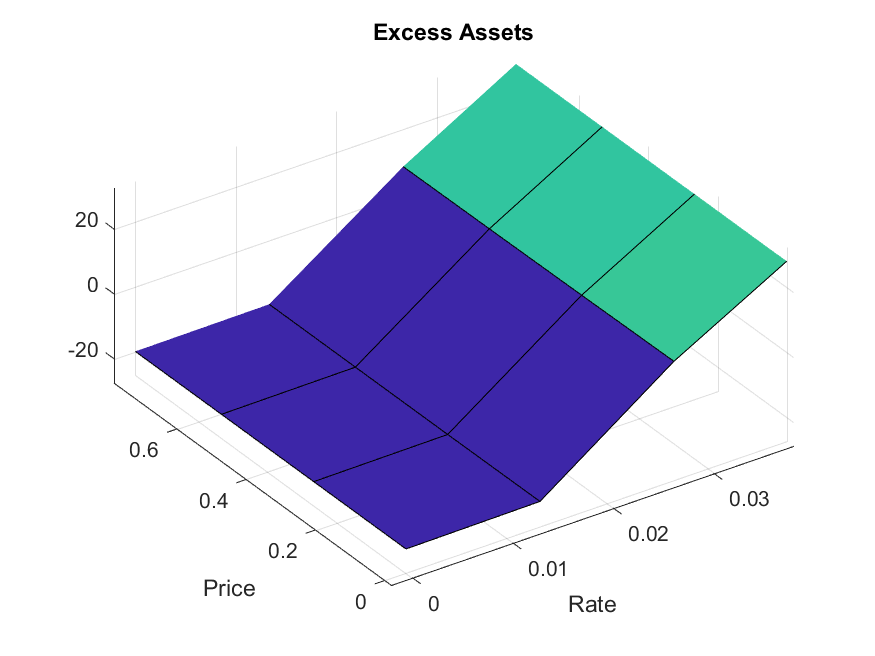
\includegraphics[angle=0,width=.5\textwidth]{figures/FIG_EQUILIBIUM1.png}\\ 
\multicolumn{2}{c}{(c) Equilibrium} \\  
%\multicolumn{2}{c}{(d) Equilibrium(repeated)} \\
%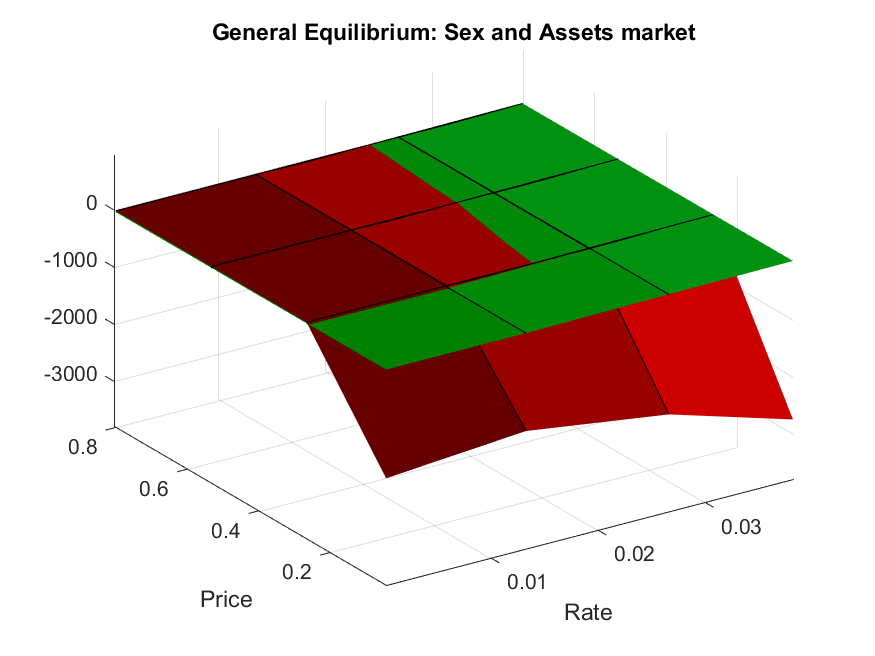
\includegraphics[angle=0,width=.5\textwidth]{figures/FIG_EQUILIBIUM3.png} 
%& 
%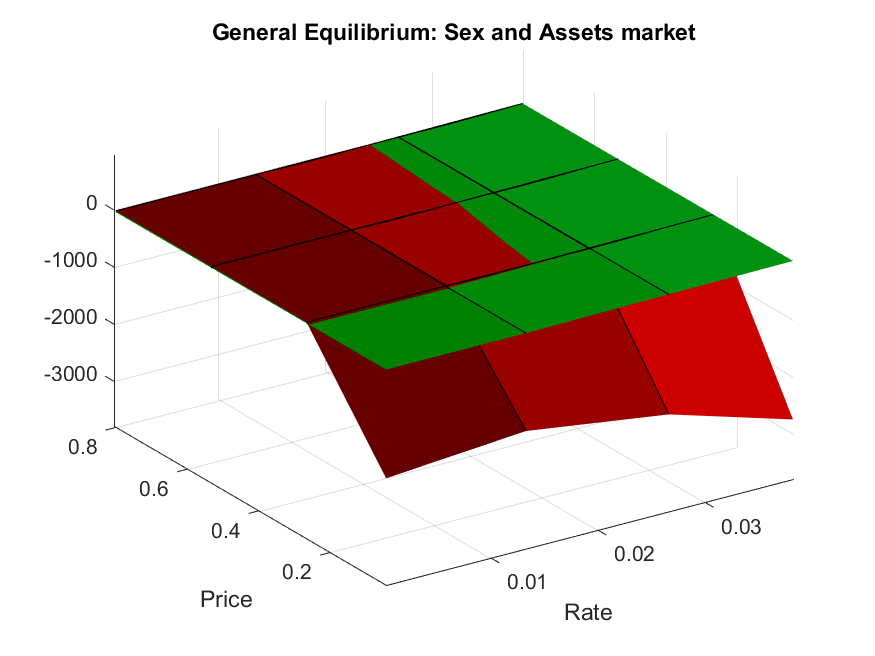
\includegraphics[angle=0,width=.5\textwidth]{figures/FIG_EQUILIBIUM3.png} 
\end{tabular}
\end{center}
\label{fig:1}
\end{figure}
%\section{Results}\label{sec6}
\begin{itemize}
\item Simulating a positive one standard deviation productivity shock on the agricultural sector:
\end{itemize}


\begin{figure}[H]
\centering
\begin{tabular}{c}
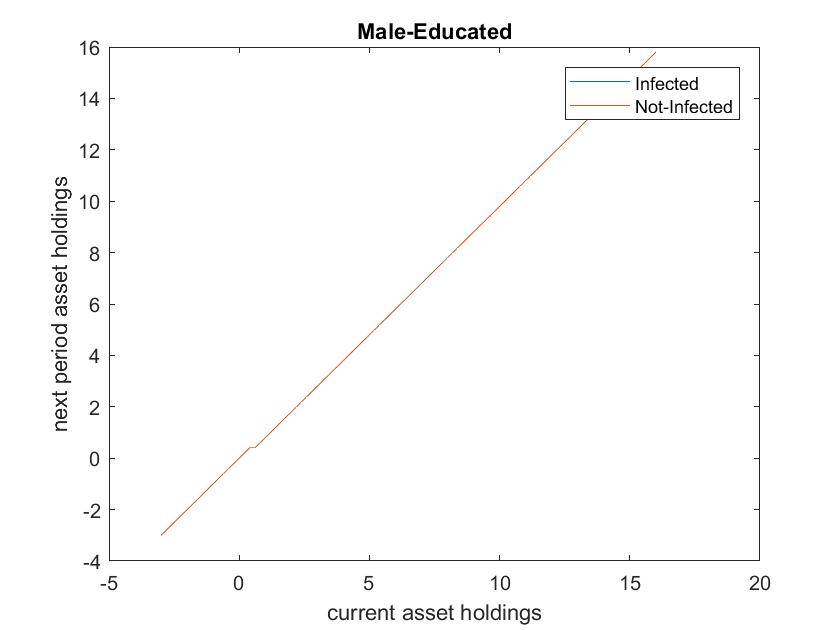
\includegraphics[width = 1\textwidth, height = 0.4\textheight]{sections/fig1.jpg}\\
\end{tabular}
\caption{Impulse response function on aggregate variables}
\label{fig1}
\end{figure}

\begin{figure}[H]
\centering
%\includegraphics[width = 15cm, height = 11cm]{sections/fig_t.jpg}\\
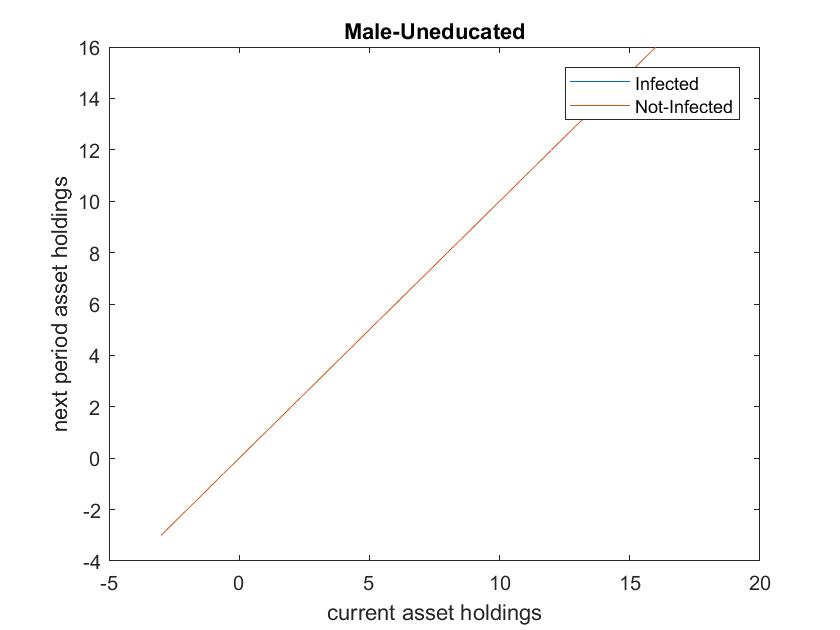
\includegraphics[width = 1\textwidth, height = 0.4\textheight]{sections/fig2.jpg}\\

\caption{Impulse response function on the agricultural sector}
\label{fig2}
\end{figure}

\begin{figure}[H]
\centering
%\begin{tabular}{c}
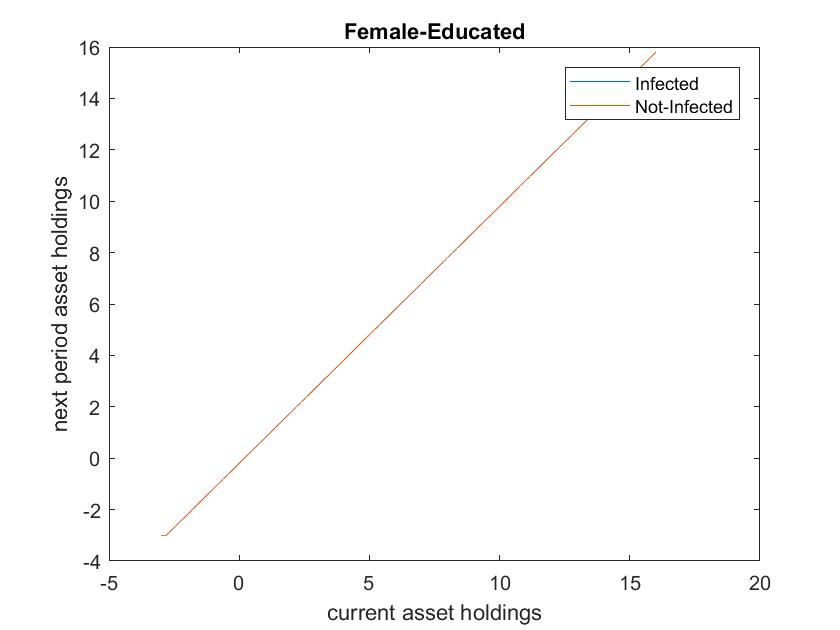
\includegraphics[width = 1\textwidth, height = 0.4\textheight]{sections/fig3.jpg}\\
%\end{tabular}
\caption{Impulse response function on the industry sector}
\label{fig3}
\end{figure}

\begin{figure}[H]
\centering
%\begin{tabular}{c}
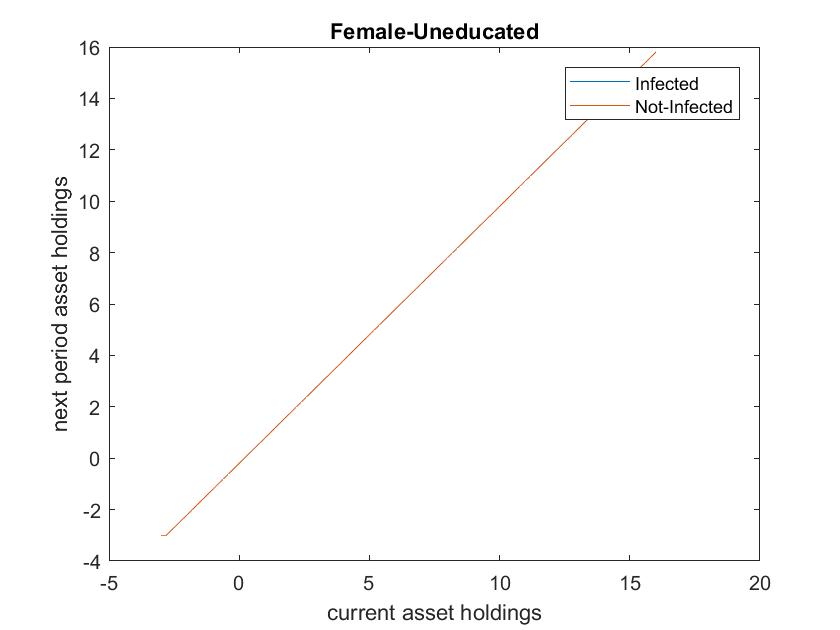
\includegraphics[width = 1\textwidth, height = 0.4\textheight]{sections/fig4.jpg}\\
%\end{tabular}
\caption{Impulse response function on the services sector}
\label{fig4}
\end{figure}

It can be seen in Figure\ref(fig2) that a positive shock on the agricultural sector, increases agricultural production and with it internal demand for inputs (co-movement) in addition the effect remains for at least two periods in the future(persistence)\footnote{it is important to note that the persistence in the model occurs by construction do to the high value of the shock auto-correlation parameter, if $\rho_{k}=0$ persistence is no longer observable}. Figure \ref{fig1} shows that the increase of agricultural production leads to an increase of total production in the economy, however, unemployment rises because employees from less productive sectors loose their jobs and are not immediately allocated to the more productive sector due to training costs.  Furthermore, an increase of the productivity in one sector will attract employment to the high productive sector, reducing the amount of people employed on the other industries, this is the case for the industry and services sector, see Figure\ref{fig3}, Figure\ref{fig4}. These results are broadly consistent with the findings in the literature on sectoral analysis \cite{long}, \cite{basu}, \cite{santoro}.

\section{Concluding Remarks}\label{conclu}
The Model presented in the following sections lacks micro-economic foundations for the inclusion of the price ratios. It therefore compulsory to switch into to a specification in which these are justified. 
The calculation of the steady state of model is extremely sensitive to slight changes in the parametrization, as the solution routine requires to input values that are close to the solution.


\newpage
\bibliography{sections/references}
%\clearpage
\newpage
%\appendix
%\section{Appendix}


\section{Solution Algorithm}

\subsection*{Computing the stationary equilibrium for the Pre-epidemic Stage 0}

\noindent \textbf{\textit{Algorithm No.1}: Computation of the stationary equilibrium:}\\

\noindent\textit{Step 1: Make initial guesses of price $p$ and interest rate $r$.\\
Step 2: Compute the agents decision rules.\\
Step 3: Compute the stationary distribution of assets (follow Algorithm No.2).\\
Step 4: Compute aggregate assets demand and aggregate sex demand. Check the aggregate consistency conditions.\\
Step 5: If conditions are not met, update $p$ and $r$ and return to Step 2.
}\\

Keep in mind that \textit{Algorithm No.1} is generic enough so that it can also be applied to compute the stationary equilibrium of any stage of the HIV epidemic.\\

For the computation of the decision rules I make use of value function iteration with linear interpolation as described in any computational methods text book\footnote{Refer to \cite{mauss}, \cite{judd}, \cite{sargent}}. For the value function iteration procedure it is necessary to choose a grid over the asset space $A=\{a_{1}=a_{min},...,a_{n}=a_{max}\}$ where $a_{min}$ and $a_{max}$ are the values chosen in the calibration. \\

\noindent\textbf{\textit{Algorithm No.2}: Computation of the invariant distribution:}\\

\noindent\textit{Step 1: Choose a grid over the asset space $A=\{a_{1}=a_{min},...,a_{n}=a_{max}\}$.\\
Step 2: Set a time iteration counter $t=0$ and choose an initial (discrete) density function $\phi_{0}(a,e,g,s)$ over the state space.\\
Step 3: Initialize $\phi_{t+1}(a',e,g,s')$\footnote{$\phi_{t+1}$ is of dimensions $n\times (m*w*q)$, where $m=2$, $w=2$ and $q=2$ since education, type and stochastic states can only be of two sorts.} and compute the optimal next period wealth $a'$ with the help of the decision rule.\\
Step 4: For all $a'\in A$, $e \in E$, $g \in G$ and $s \in S$compute the following expression:}
\begin{align}\label{eq:10}
    \phi_{t+1}(a',e,g,s')=\sum_{a,e,s}\sum_{s'|s}\textbf{1}_{a'\in\mathcal{A}}\gamma_{e}\pi(s'|s)\phi_{t}(a,e,g,s) + \psi_{e}\phi_{t}(a',e,g,s')
\end{align}
\textit{
Step 5: If $|\phi_{t+1}-\phi_{t}|<exp(-12)$ stop, otherwise set $\phi_{t}=\phi_{t+1}$ and return to Step 3.}\\

For simplicity reasons the grid chosen for \textit{Algorithm No.2} is the same as the grid chosen for the value function iteration procedure in \textit{Algorithm No.1}, otherwise if the grid would be finer it would be necessary to include the probabilities of $a'(a,e,g,s)$ falling between the respective points in the grid.\\

For \textit{Step2} of \textit{Algorithm No.2} I choose the uniform distribution as the initial values of the distribution. The algorithm should converge regardless of the choice of the initial distribution.


\subsection*{Computing the stationary equilibrium for Stage 1}

\textbf{Solving the Miopic stage}\\
Computation of transition dynamics to a new steady state at every point in time.\\
\noindent \textbf{\textit{Algorithm No.3}: Computation of the Myopic stage:}\\


We are after a sequence of $g_1$. To get each of them we need to solve for the entire transition.

At each period $\tau \in \{T_0+1,..., \infty\}$, agents get a permanent unexpected shock to $\gamma_m$ and $\pi_m$. Then, we need to solve the following algorithm %for each period $t$, that is, every time (which is every period) individuals receive an unexpected shock:\\

\begin{itemize}
\item Step 0: Set $\tau=T_0+1$,
\item Step 1: Compute the recursive stationary equilibrium of the Myopic stage associated with the new $\gamma_m$ and $\pi_m$.
\item Step 2: Choose a very large number of transition  periods $(T-\tau)$.
\item Step 3: Compute the equilibrium transition dynamics from the stationary equilibrium in item 1 (i.e., at $T$) to the  equilibrium in period $\tau$. We compute this standardaly going backwards.
\item Step 4: Stop if $\tau=T_1$
\item Step 5: Replace $\tau=\tau+1$ and go back to Step 1.
\end{itemize}


\subsection*{Computing the stationary equilibrium for Stage 2}
\noindent \textbf{Solving the Maturity of the Epidemic}

Computation of the transition dynamics by guessing a finite-time path for prices.\\

\noindent \textbf{\textit{Algorithm No.3}: Computation of the transition to the Maturity Stage:}\\

\begin{itemize}
\item Step 1: Choose the number of transition periods ($T_2-T_1$) that go from the last  period in Stage 1 (HIV Myopia) ($t=T_1$) to the recursive stationary equilibrium of Stage 2 of the epidemic (HIV Maturity) ($t=T_2$).
\item Step 2: Compute the recursive stationary equilibrium of Stage 2 of the epidemic. This stationary equilibrium is associated with $\lim_{t \rightarrow \infty }\widetilde{\rho}_{e,t}=\rho$. That is, in the stationary equilibrium both education groups have completed learning of the true probability of how HIV risk as a function of sex.
\item Step 3: Guess a time path for the prices $p_{t}$ and $r_{t}$, and a time path for beliefs $\widetilde{\rho}_{e,t}$ by education group.
%The values of these variables in the first period $t = 0$ and last period $t = T$ are implied by the last distribution of the myopic stage of the epidemic and the recursive stationary equilibrium associated with $\widetilde{\rho}_{e,t}=\rho$, i.e., complete learning of the true probability of HIV infection for both education groups.
%\item Step 4: Make an initial guess of $\widetilde{\rho_{e,t}}$ for each education group. and iterate on Bayes rule to generate an exogenous learning path for $ \rho_{t}$ until $T$.
\item Step 5: Compute the equilibrium policy (and value) functions iterating backwards in time, $t = T_2-1,...,T_1$.
\item Step 6: Simulate the evolution of the distribution with the help of the optimal policy functions and the initial distribution for the transition from $t = T_1$ to $t = T_2$.
\item Step 7: Compute the time path of net asset level and excess demand for sex. If markets don't clear along the path, then return to step 3.
\item Step 8: Compare the simulated distribution  with the stationary distribution function. If they are not the same try increasing the horizon $T$.
\end{itemize}


%\subsection*{Computing the dynamics for the pre-epidemic stage}













\subsection{Pre-Epidemic graphs}
\begin{figure}[H]
\caption{Policy Functions Educated Buyers}
\hspace{-2.0cm}
\begin{center}
\begin{tabular}{cc}
\multicolumn{1}{c}{(a) Value function} &  
\multicolumn{1}{c}{(b) Assets function} \\
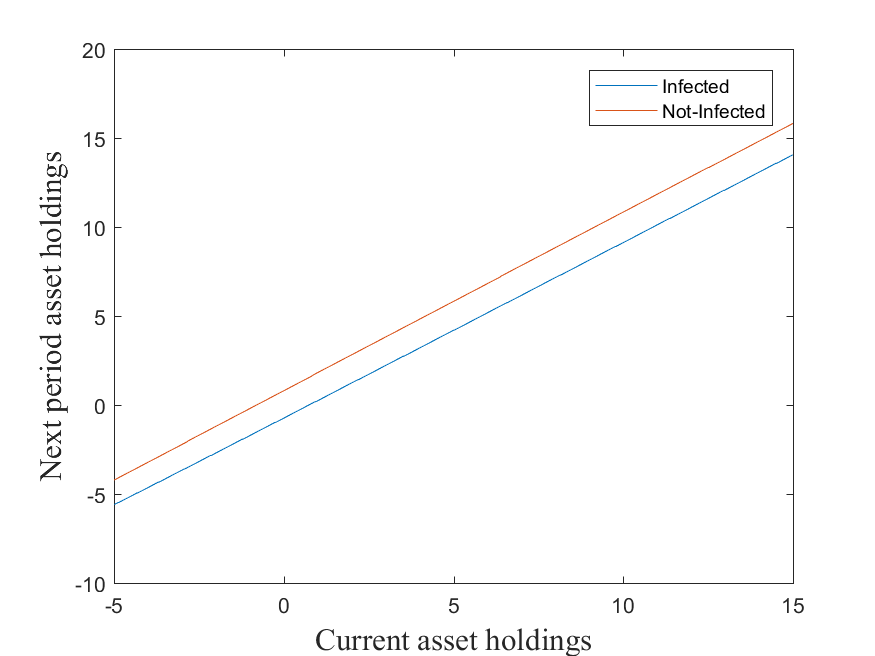
\includegraphics[angle=0,width=.5\textwidth]{figures/FIG1.png}   & 
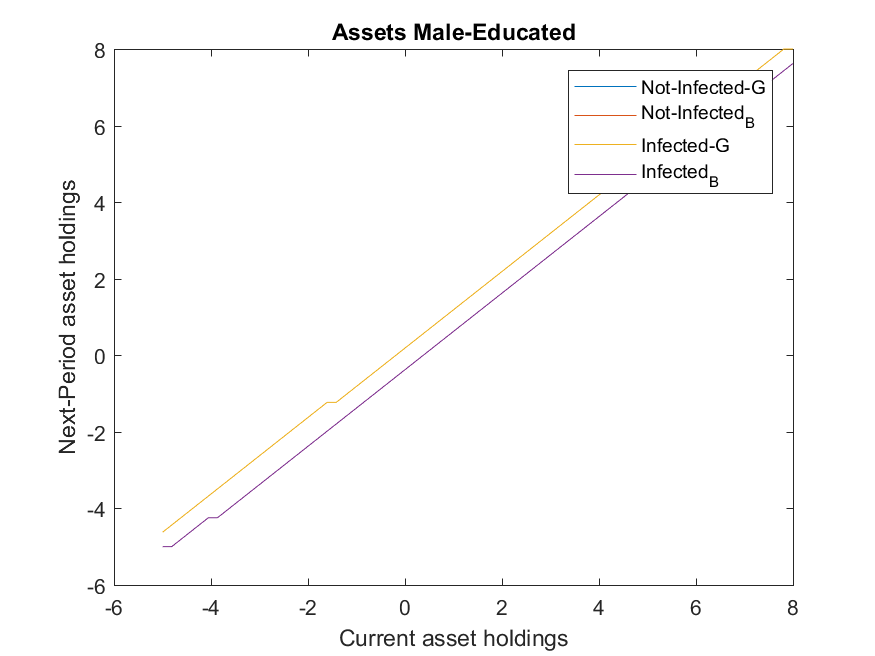
\includegraphics[angle=0,width=.5\textwidth]{figures/FIG3.png} \\
\multicolumn{1}{c}{(c) Consumption function} &  
\multicolumn{1}{c}{(d) Sex consumption function } \\
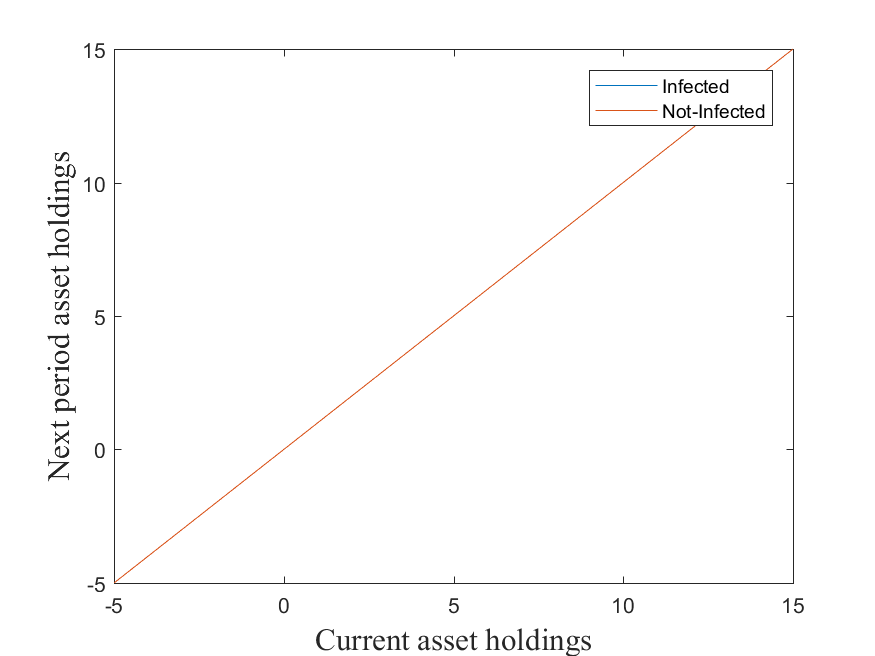
\includegraphics[angle=0,width=.5\textwidth]{figures/FIG2.png}   & 
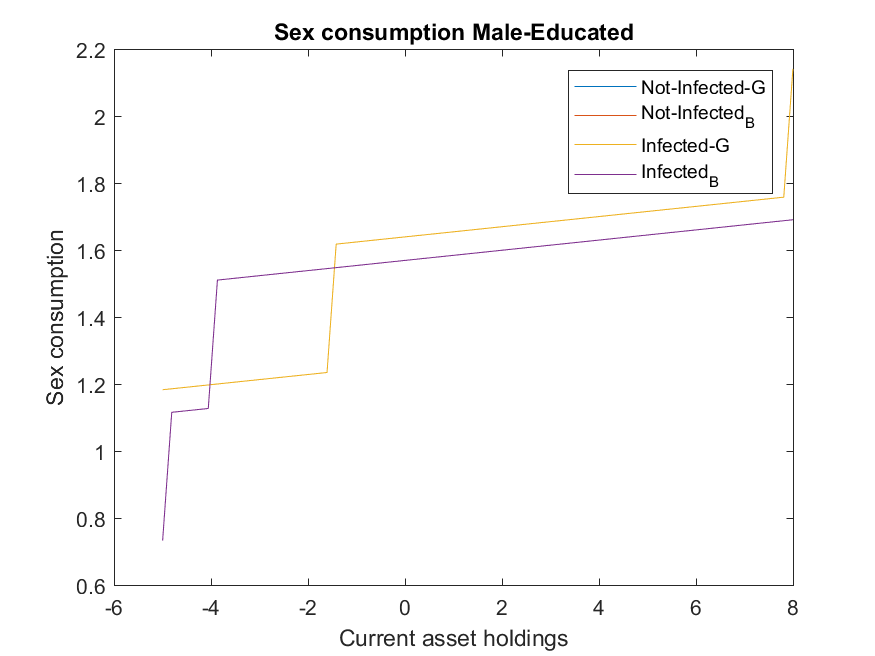
\includegraphics[angle=0,width=.5\textwidth]{figures/FIG4.png} \\
%\multicolumn{1}{c}{(a) Value function} &  
%\multicolumn{1}{c}{(b) Assets function} \\
\end{tabular}
\end{center}
\label{fig:2}
\end{figure}

\begin{figure}[H]
\caption{Policy Functions Educated Sellers}
\hspace{-2.0cm}
\begin{center}
\begin{tabular}{cc}
\multicolumn{1}{c}{(a) Value function} &  
\multicolumn{1}{c}{(b) Asset function} \\
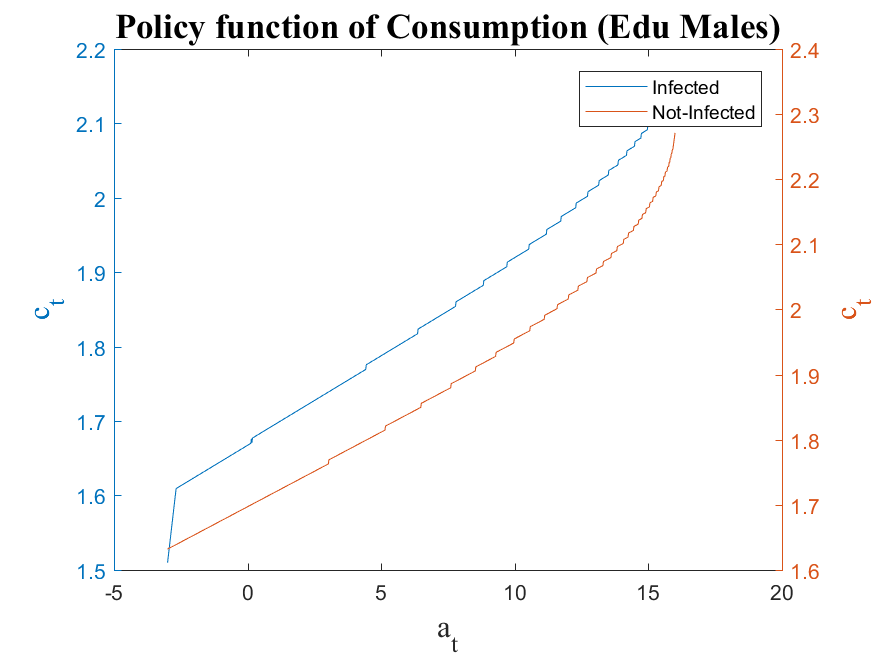
\includegraphics[angle=0,width=.5\textwidth]{figures/FIG5.png}   & 
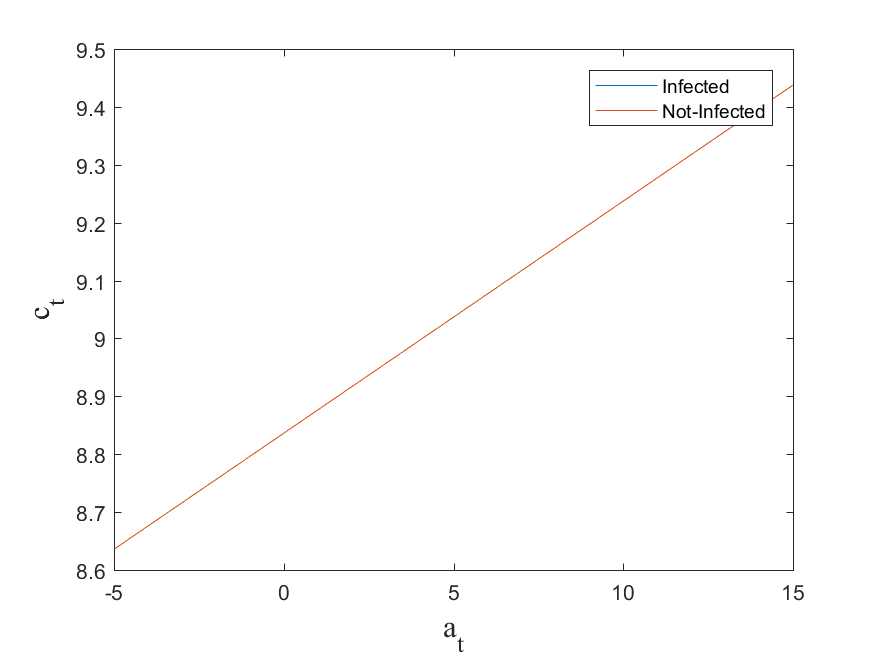
\includegraphics[angle=0,width=.5\textwidth]{figures/FIG7.png} \\
\multicolumn{1}{c}{(c) Consumption function} &  
\multicolumn{1}{c}{(d) Sex Production function } \\
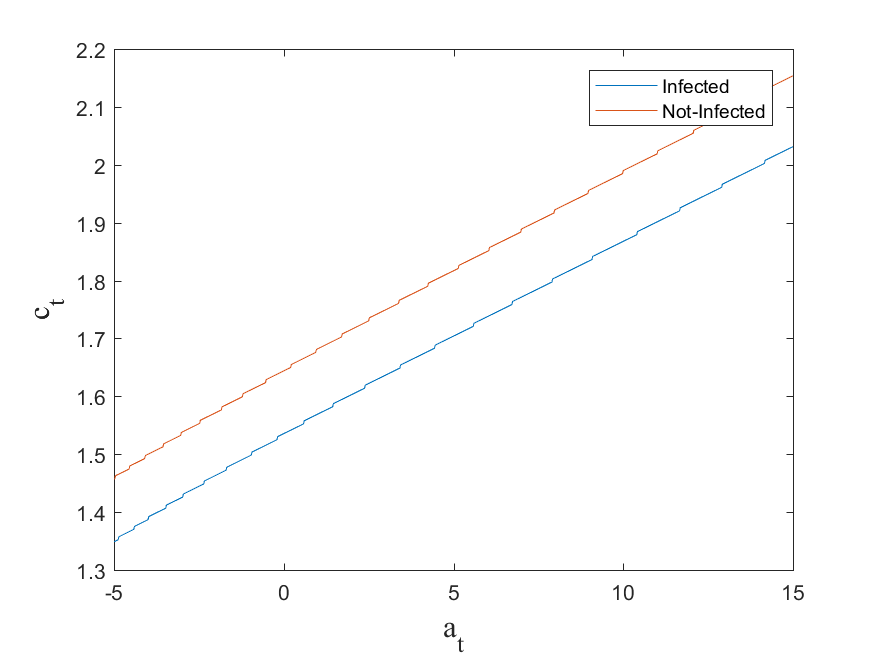
\includegraphics[angle=0,width=.5\textwidth]{figures/FIG6.png}   & 
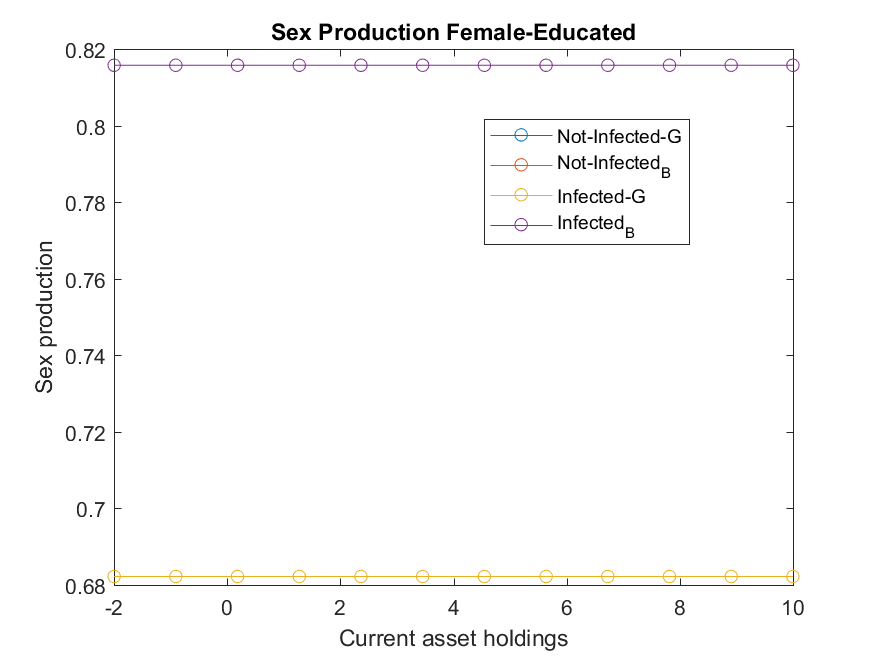
\includegraphics[angle=0,width=.5\textwidth]{figures/FIG8.png} \\
\end{tabular}
\end{center}
\label{fig:3}
\end{figure}



\begin{figure}[H]
\caption{Comparison plots}
\hspace{-2.0cm}
\begin{center}
\begin{tabular}{cc}
\multicolumn{1}{c}{(a) Asset Policy Functions} &  
\multicolumn{1}{c}{(b) Consumption Policy Functions} \\
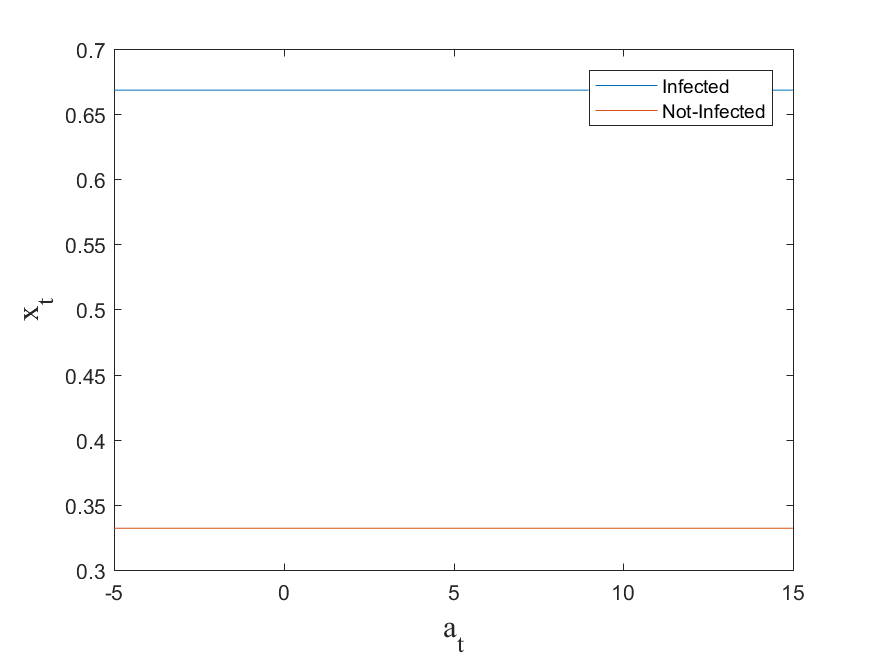
\includegraphics[angle=0,width=.5\textwidth]{figures/FIG11.png}   & 
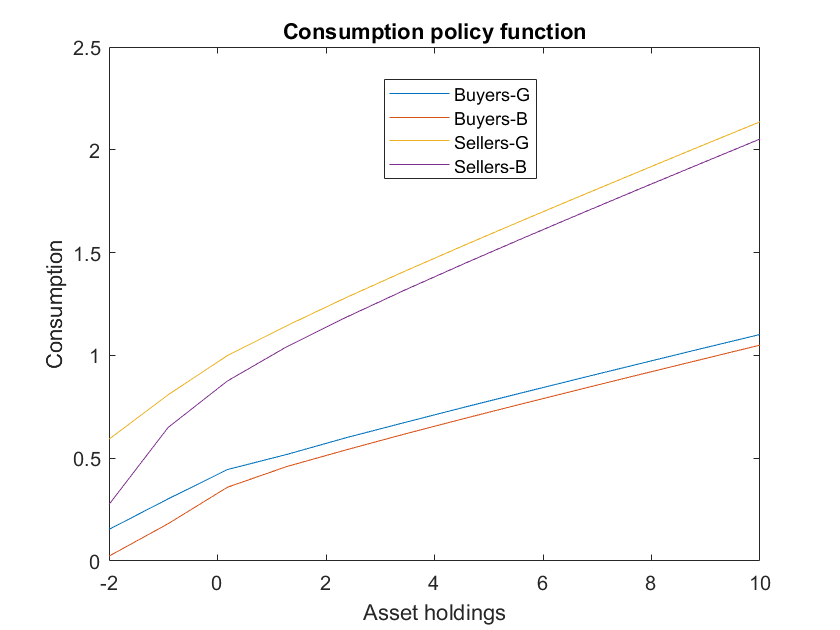
\includegraphics[angle=0,width=.5\textwidth]{figures/FIG12.png}\\ 
\multicolumn{2}{c}{(c) No Capital Income} \\  
%\multicolumn{2}{c}{(d) Equilibrium(repeated)} \\
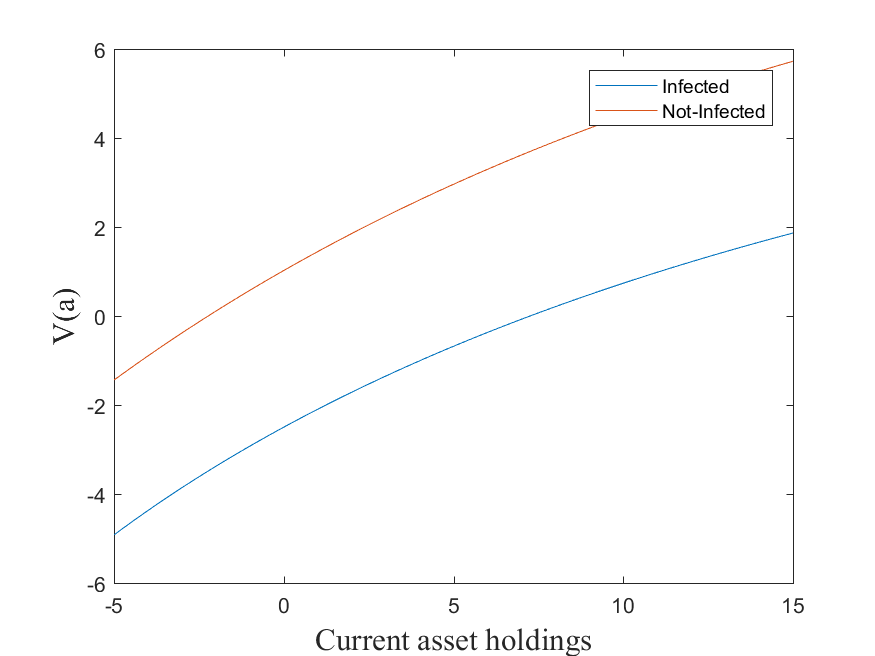
\includegraphics[angle=0,width=.5\textwidth]{figures/FIG13.png} 
%& 
%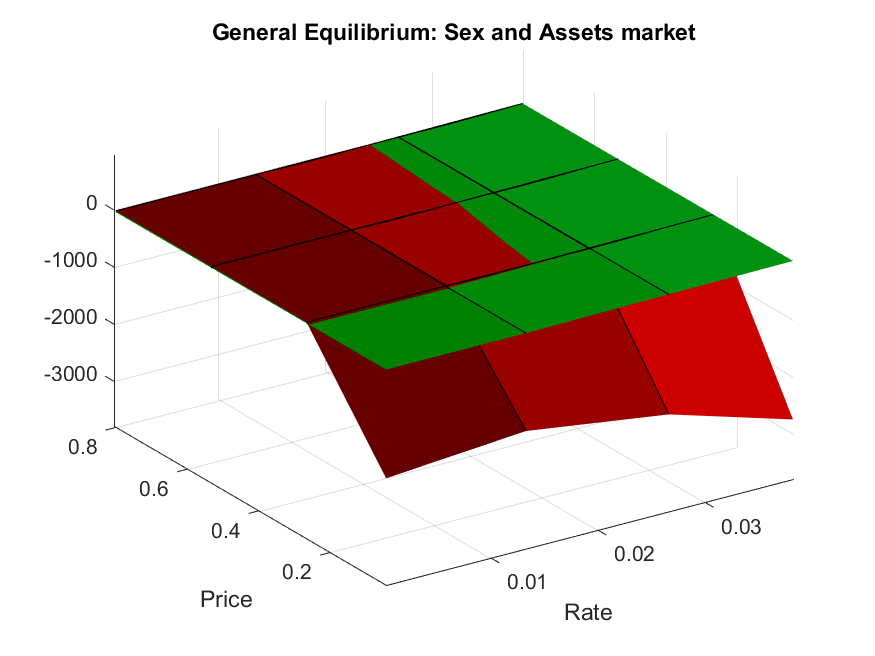
\includegraphics[angle=0,width=.5\textwidth]{figures/FIG_EQUILIBIUM3.png} 
\end{tabular}
\end{center}
\label{fig:5}
\end{figure}
\end{document}





%%%%%%%%%%%%%%%%%%%%%%%%%%%%%%%%%%%%%%%%%%%%%%%%%%%%%%%%%%%
%\end{comment}

